\documentclass{egpubl}
\usepackage{eg2014}

\usepackage[utf8]{inputenc}
\usepackage[T1]{fontenc}

\ConferencePaper
\electronicVersion

\ifpdf \usepackage[pdftex]{graphicx} \pdfcompresslevel=9
\else \usepackage[dvips]{graphicx} \fi

\let\bibhang\arealyundefinedcommand
\usepackage[backend=bibtex, bibencoding=ascii, safeinputenc, style=alphabetic]{biblatex}
\usepackage{csquotes}

\makeatletter
\renewcommand{\electronic@Version}{%
   \usepackage[pdftex,
    %pagebackref=true,
    colorlinks,linkcolor=blue,citecolor=blue,urlcolor=blue,
    bookmarks=false,
    pdfpagemode=UseNone,
    pdftitle={\@shorttitle},
    pdfauthor={\@shortauthor},
    pdfsubject={\pdf@Subject},
    pdfkeywords={Computer Graphics Forum, EUROGRAPHICS}]{hyperref}
  }
\renewcommand{\printed@Version}{%
   \usepackage[pdftex,
    %pagebackref=false,
    colorlinks,linkcolor=black,citecolor=black,urlcolor=black,
    bookmarks=false,
    pdfpagemode=UseNone,
    pdftitle={\@shorttitle},
    pdfauthor={\@shortauthor},
    pdfsubject={\pdf@Subject},
    pdfkeywords={Computer Graphics Forum, EUROGRAPHICS}]{hyperref}
  } 
\makeatother  
\electronicVersion
\PrintedOrElectronic

% prepare for electronic version of your document
\usepackage{t1enc}
\usepackage{dfadobe}

\usepackage{egweblnk}

% Fix the invalid paperheight warning
\setlength{\paperheight}{11in}



%%%%%%%%%%%%%%%%%%%%%%%%%%%%%%%%%%%%%%%%%%%%%%%%%%%%%%%%%%%%%%
\usepackage[english]{babel}
\usepackage{ragged2e}

% Math
\usepackage{mathtools}
\usepackage{amsmath}
\usepackage{amsfonts}
\usepackage{amssymb}
\newcommand{\Real}{\ensuremath{\mathbb{R}}}

%Floats
\usepackage{graphicx}
% \usepackage[hang, small,labelfont=bf,up,textfont=sl,up, justification=raggedright]{caption}
\usepackage{subcaption}
\DeclareCaptionLabelFormat{opening}{(#2)}
\captionsetup{subrefformat=opening}

% References within paper
\usepackage{varioref}
\usepackage{hyperref}
\usepackage[noabbrev, capitalise, nameinlink]{cleveref}

% Lists
\usepackage{enumitem}

% \hyperref[sec:intro]{Appendix~\ref*{sec:intro}}


\newcommand{\crefs}[1]{\hyperref[#1]{Section~\ref*{#1}}}
\newcommand{\Crefs}[1]{\hyperref[#1]{Section~\ref*{#1}}}

\newcommand{\crefe}[1]{\hyperref[#1]{Equation~\ref*{#1}}}
\newcommand{\Crefe}[1]{\hyperref[#1]{Equation~\ref*{#1}}}

% Temporary
\usepackage{todonotes}
\newcommand{\laura}[1]{\todo[inline, color=red]{\textbf{Laura:} #1}}
\newcommand{\rick}[1]{\todo[inline, color=green]{\textbf{Rick:} #1}}
\newcommand{\future}[1]{\todo[inline, color=yellow]{\textbf{Possibly eventually:} #1}}
\newcommand{\plaatje}[1]{\todo[inline, color=blue!20]{\textbf{Plaatje:} #1}}
\newcommand{\ooit}[1]{\todo[inline, color=green!20]{\textbf{(n)ooit:} #1}}

\usepackage{etoolbox}
\newtoggle{PHONG}
\togglefalse{PHONG}


% Settings for header
\title[PN Triangles]%
      {A Discussion of Curved Point-Normal Triangles}

\author[R. van Veen \& L. Baakman]
       {R. van Veen\thanks{These authors contributed equally to this work.}$^{1}$
        and L.\,E.\,N. Baakman\footnotemark[1]$^{1}$
        \\
         $^1$Computing Science Department of the University of Groningen
       }

\addbibresource{content/biblio.bib}


\usepackage{xprintlen}

\begin{document}
	

\todo[inline]{Subdivide vervangen met tesselation}
% \laura{Add doi file and url to the bibliography}

\listoftodos

%!TEX root = ../main.tex

\teaser{
	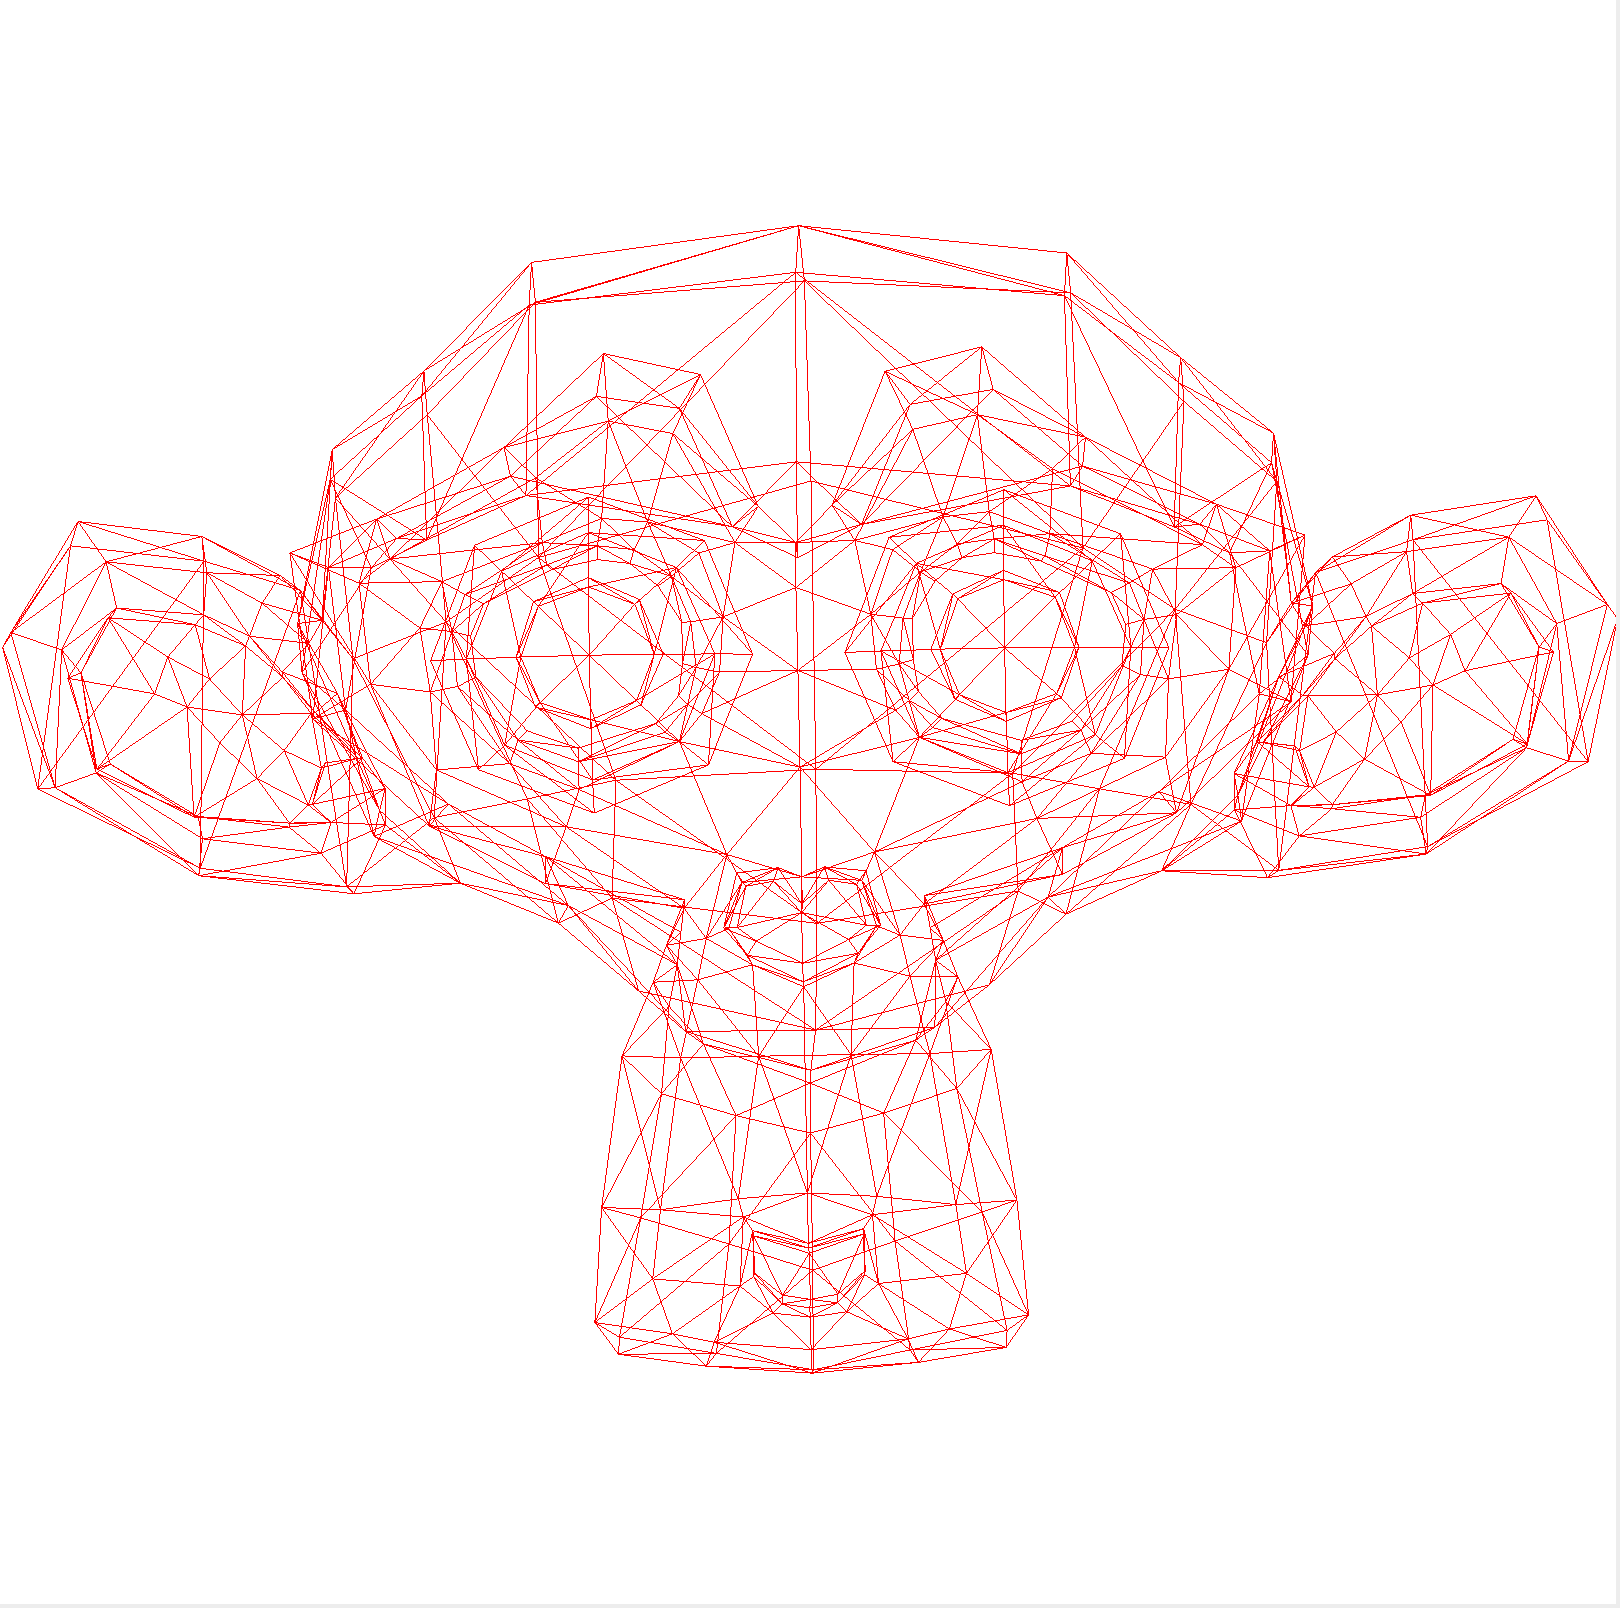
\includegraphics[width=0.32\linewidth]{content/img/header/Suzanne_wireframe.png}
	
\includegraphics[width=0.32\linewidth]{content/img/header/Suzanne.png}
	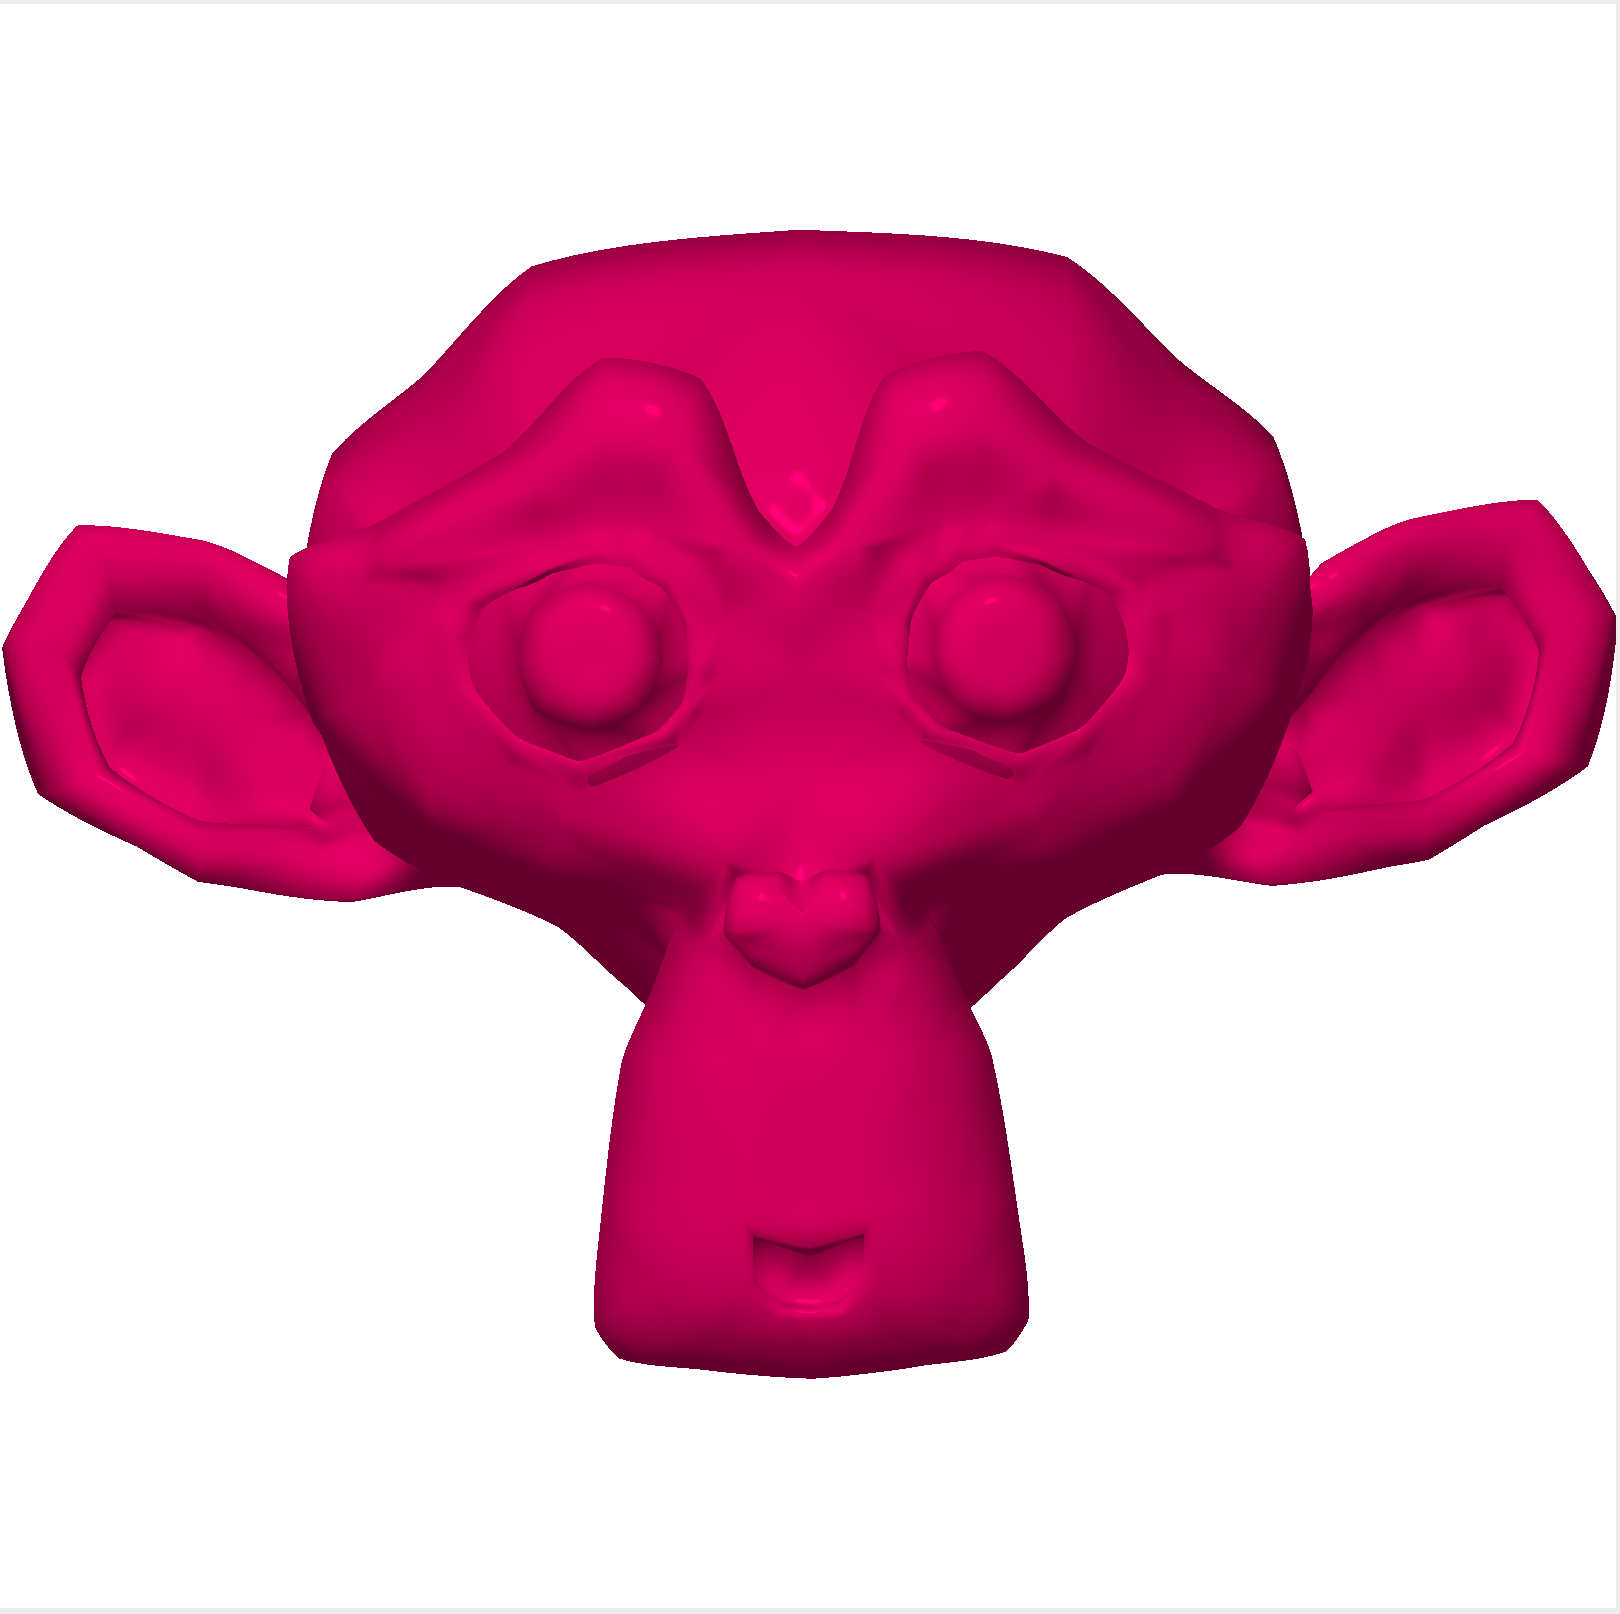
\includegraphics[width=0.32\linewidth]{content/img/header/Suzanne_PN.png}
	\centering
	\caption{From left to right: the triangular input mesh, the Phong shaded mesh, and the {Phong shaded mesh using point normal triangles and an inner and outer tessellation level of $12.0$.}
	\label{fig:preamble:teaser}
}

\maketitle

%!TEX root = ../main.tex

\begin{abstract}
	\citeauthor{vlachos2001curved} introduced point-normal triangles in \citeyear{vlachos2001curved} to improve the visual quality of triangle meshes in a fast way on the CPU, without having to change the mesh. Since then a lot of changes have been made to the OpenGL pipeline, making it possible to render with point-normal triangles on the GPU. 

	% Wat gaan we doen % Wat is eruit gekomen: CPU/GPU
	We discuss how one can implemented point-normal triangles on the GPU and discuss the differences with the CPU implementation. We have found that there are probably no differences.

	% Wat gaan we doen % Wat is eruit gekomen: normals
	Further more we also consider the use of normals based on the geometry, `real' normals, instead of the quadratically varying normals, `fake' normals, proposed by \citeauthor{vlachos2001curved}. We have concluded that although the resulting normal fields are the same the `fake' normals are computationally less expensive, and thus preferably.
	~\\

	\begin{classification}
		% Take a look at: http://academia.stackexchange.com/questions/15252/is-the-new-acm-2012-taxonomy-usable-in-use
		% \ccsdesc[500]{Computing methodologies~Parametric curve and surface models}
		\CCScat{Computer Graphics}{I.3.3}{Shape modeling}{Parametric curve and surface modeling}
	\end{classification}
\end{abstract}

% \printlen[3][cm]{\columnwidth}
% \the\columnwidth

%!TEX root = ../main.tex

\section{Introduction}

\todo[inline]{Context: Why PN triangles: fast smooth real-time rendering}
\todo[inline]{Context: global idea of PN triangles}
\todo[inline]{Context: global idea of phong tesselation}
\todo[inline]{Context: relationship between phong and pn}

\todo[inline]{Application Domain: useful for real time rendering, not for CAD, explain why not....}

\todo[inline]{Required Background knowledge: nothing comes to mind, currently}

\todo[inline]{Explain structure of report}


%!TEX root = ../main.tex
\section{Problem Definition}
\label{s:problem}
We consider a number of sub problems associated with point-normal triangles.

\begin{enumerate}[label=(\roman*)]
	\item \label{it:problem:fakeNormals}
		% Waarom willen we het weten
		In the introduction we have mentioned that point-normal triangles are not suitable for rendering in computer aided designed software, due to the `fake' normal field, as the normal component of the PN triangle does not accurately represent the actual normals. Adapting the PN triangle algorithm to use `real' normals, expands its application domain to include rendering for CAD software.
		%
		% Wat willen we weten
		However it is possible to compute the `real' normals of the vertices of the subdivided PN-triangle, using the method we present in section \ref{sss:method:normals:realNormals}. 
		%
		%Wat gaan we meten
		In this paper we compare both the computational and the visual performance of the `real' and `fake' normals. 
		% Wat verwachten we
		We do not expect a large difference in visual performance when `real' normals are used. Nor do we suppose that computing the normals based on the geometry will have a significant impact on the computational complexity of point-normal triangles.

\iftoggle{PHONG}{
	\item \label{it:problem:CompareWithPhongTesselation}
		\future{2: Compare PN triangles with phong tesselation on the following aspects: performance, continuity, visual. We try to answer the question: When use PN when Phong?}
}	

	\item \label{it:problem:GPUImplementation}
		%Waarom willen we het weten
		One major advantage of PN-triangles at the time of its introduction (\citeyear{vlachos2001curved}) was its speed. Since then geometry and tessellation shaders have been introduced into the OpenGL pipeline. 
		%
		% Wat willen we weten
		We investigate which changes have to be made to the point-normal triangles as proposed by \citeauthor{vlachos2001curved} to fit into a recent OpenGL pipeline (version 4.1).
		%
		% Hoe gaan we het meten
		In this paper we discuss the changes between the CPU implementation proposed by \citeauthor{vlachos2001curved} and our GPU implementation. 
		%
		% Wat verwachten we
		We expect that due to their locality point-normal triangles are extremely suited for computation on the GPU. Allowing us to subdivide triangular meshes faster than is possible on the CPU. 
\end{enumerate}

%!TEX root = ../main.tex

\section{Method}
\label{s:method}
\laura{Read: specifically the intro. I mention the inner and outer tessellation again, so we can reference where this is discussed. We can also leave this out, but that would leave the reader in the dark where to get that information (given that he/she starts reading at the method section, else it would have been mentioned in the introduction maybe...)}
% \todo[inline]{Global idea of PN triangles, lit less global than in introduction}
The main goal of PN triangles is to improve the visual quality of rendered models, and to do this on resource-limited hardware environments where e.g. no information about neighboring triangles can be accumulated. We ask the reader to have a look at \cref{fig:preamble:teaser}, with the following question in mind: Which rendering do you prefer? The center and right images both show a rendering using phong shading and llumination. The only difference being, that the right image is rendering using PN triangles, with an inner and outer tessellation level of $12.0$, the meaning of the tessellation level is discussed in \crefs{s:implementation}. The goal of point-normal triangles more precisely is ``to soften triangle creases and improve the visual appeal by generating smoother silhouttes and better shading'' \cite{vlachos2001curved}. \citeauthor{vlachos2001curved} mention, besides the visual improvements, the following benefits:

\begin{enumerate}[label=(\roman*)]
 	\item 
 		Point-normal triangle construction is \textit{compatible} with the existing graphics API data structures, i.e., vertex arrays together with triangle index streams, where the triangles arrive in unpredictable order.
 	\item 
 		The models are \textit{backward compatible} with hardware that does not support point-normal triangles, with minimal or no changes needed to existing models.
 	\item 
 		No setup of the application, API, or hardware driver is needed. Specifically, hardware should not be able to provide random access to neighboring primitives. Consequently the only possible communicated information between primitives are provided by using shared normals at the vertices. This does restrict the models to be rendered somewhat, as discussed in \crefs{sss:method:geometric:properties}.
 	\item 
 		Point-normal triangles are applicable to meshes with \textit{arbitrary topology}.
 	\item 
 		PN-triangle rendering is \textit{fast} and done via \textit{simple implementation} in hardware on the CPU in 2001. At the time of writing of this report, even faster execution is possible by using programmable tessellation shaders on the GPU.
 \end{enumerate} 

In the remaining part of this section we discuss the construction of point-normal triangles conceptually as well as mathematically. As mentioned in the introduction, a PN triangle is split in two different components: we refer to \crefs{ss:geometric_component} for a discussion on the geometric component and to \crefs{ss:normal_component} for the review of the normal component.

\begin{figure}
	\centering
	\plaatje{Splits in twee losse plaatjes met subfigure.}
	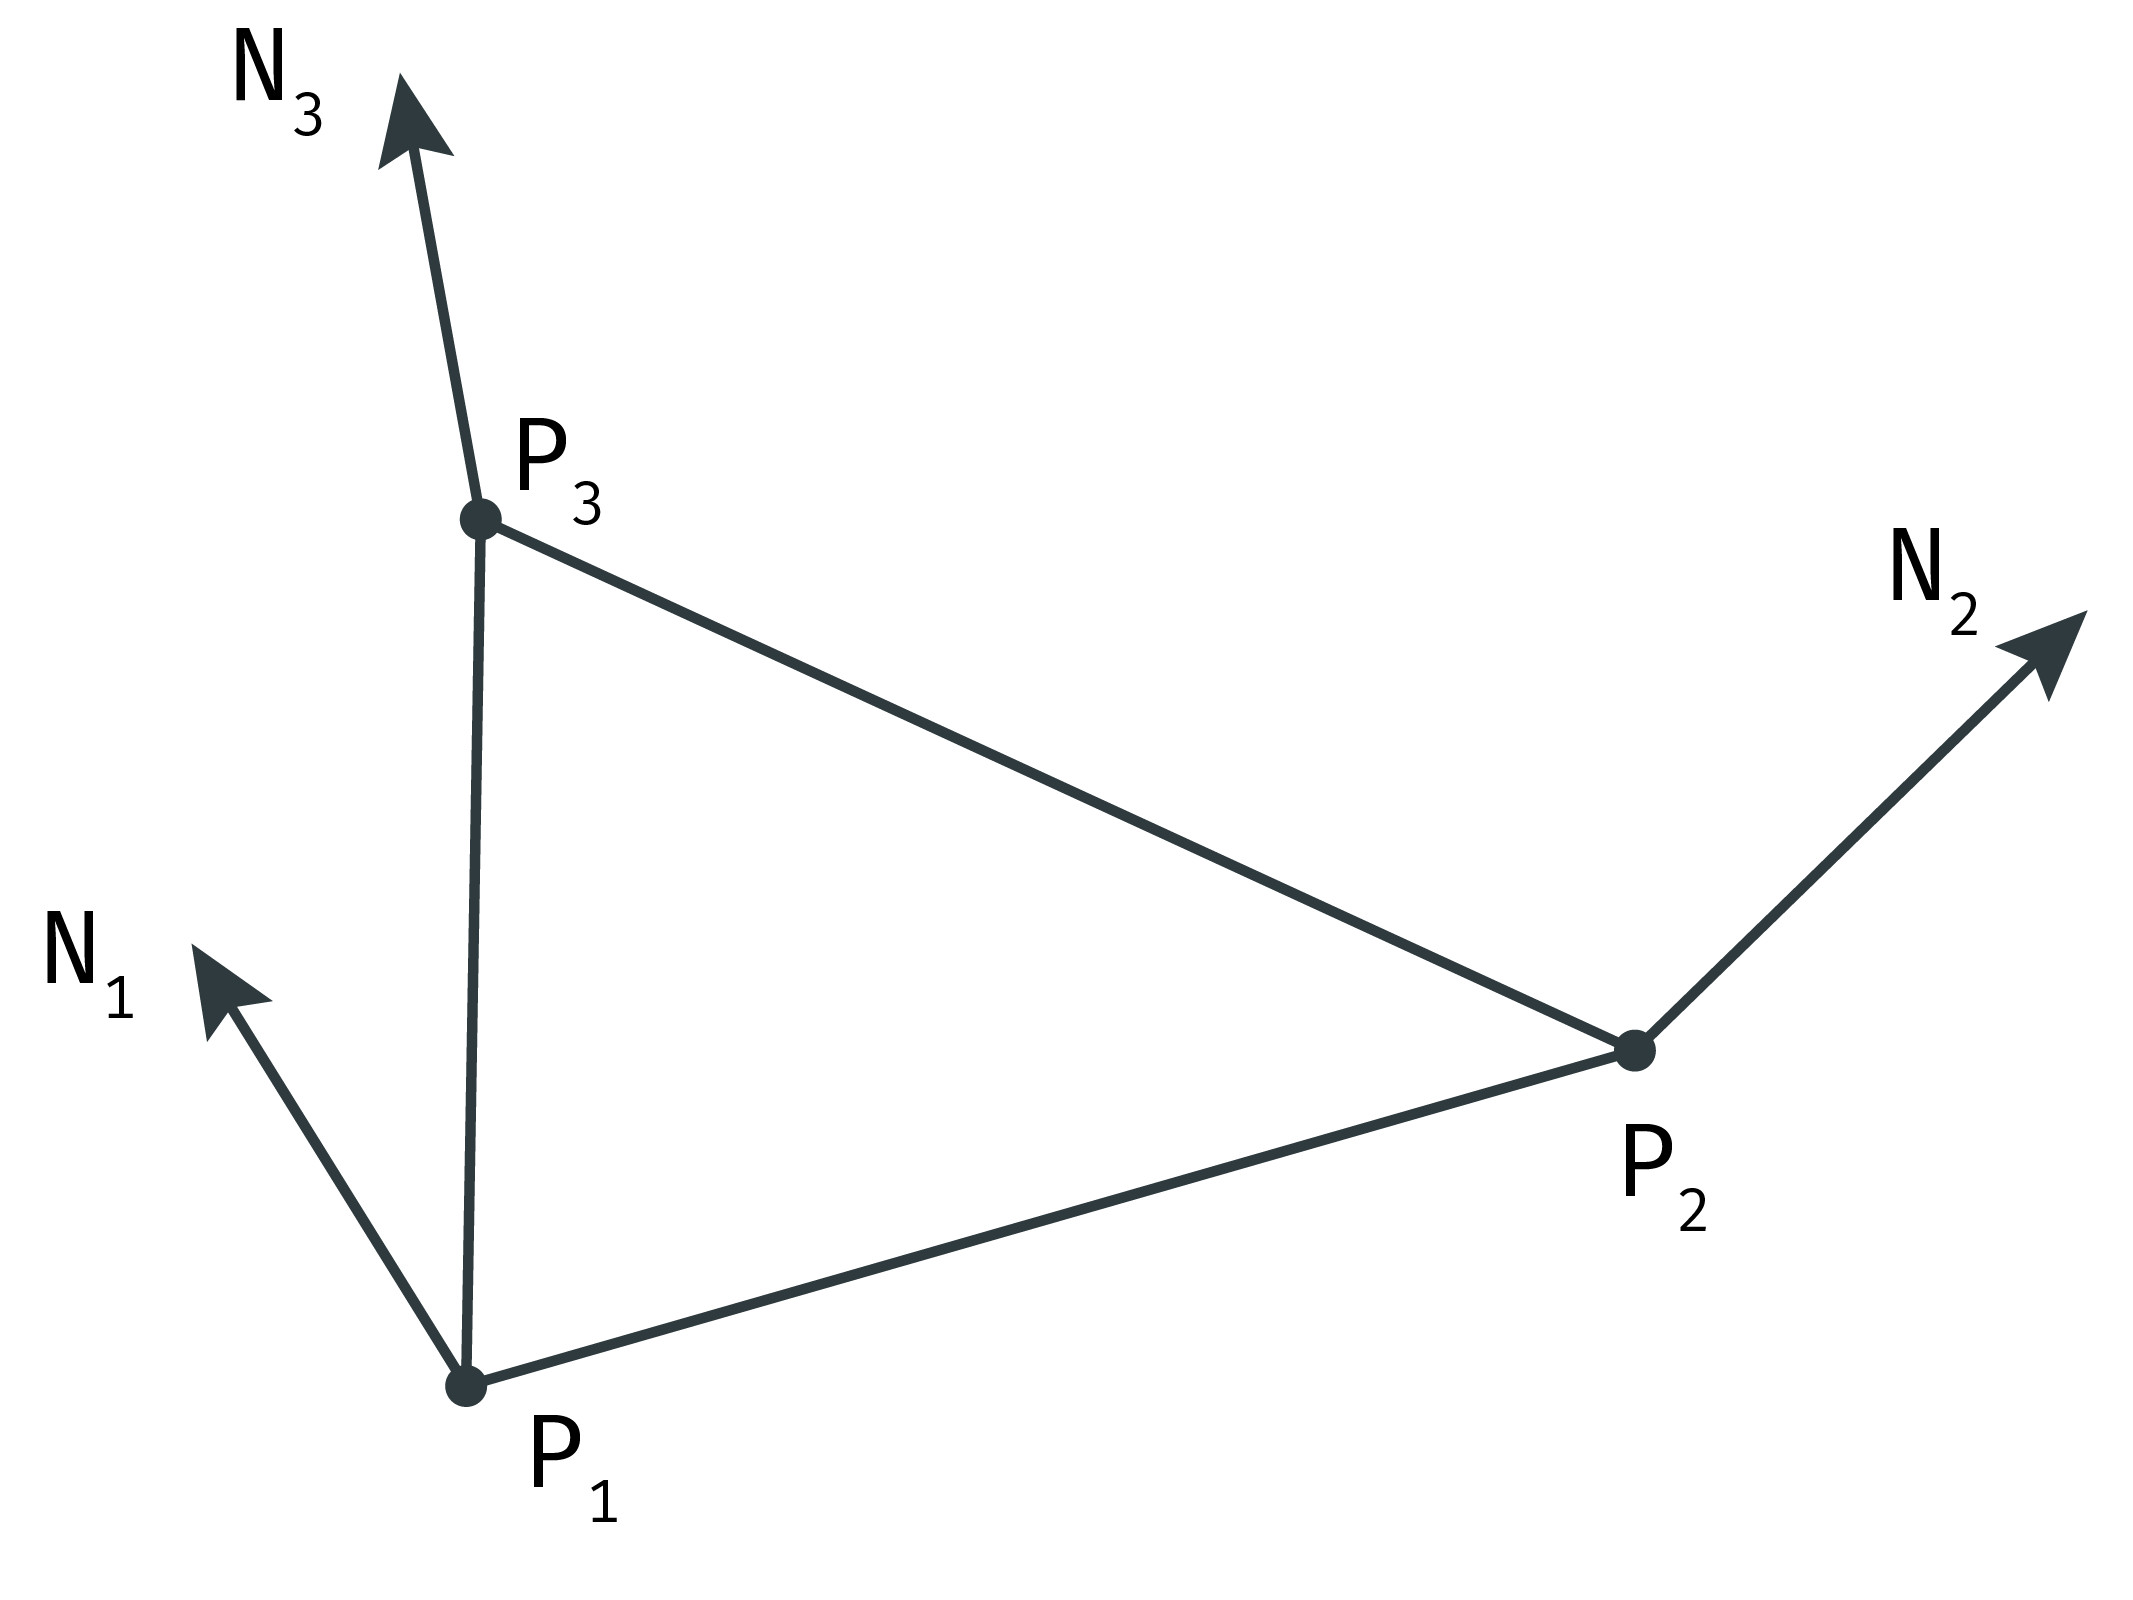
\includegraphics[width=0.45\textwidth]{./content/img/method/input.png}
	\caption{An input primitive as used by point-normal triangle consists of three vertices and three vertex normals. Note that only the information from a single primitive is used during the construction of both the geometric and the normal component.}
	\label{fig:method:input_primitive}
\end{figure}

%!TEX root = ../main.tex

\subsection{Geometric component}
\label{ss:geometric_component}
Let us emphasize again that the only used information for the construction of the geometric and normal component are the three vertices with associated normals, that define a single primitive. The vertices contain the vertex \textit{xyz}-coordinates together with a unique shared normal per vertex, i.e., the normal of each vertex is the same for every primitive using that vertex. Figure \ref{fig:method:input_primitive} shows an illustration of an input primitive. Each point-normal triangle construction starts with an input primitive of this form.

\begin{figure}
	\centering
	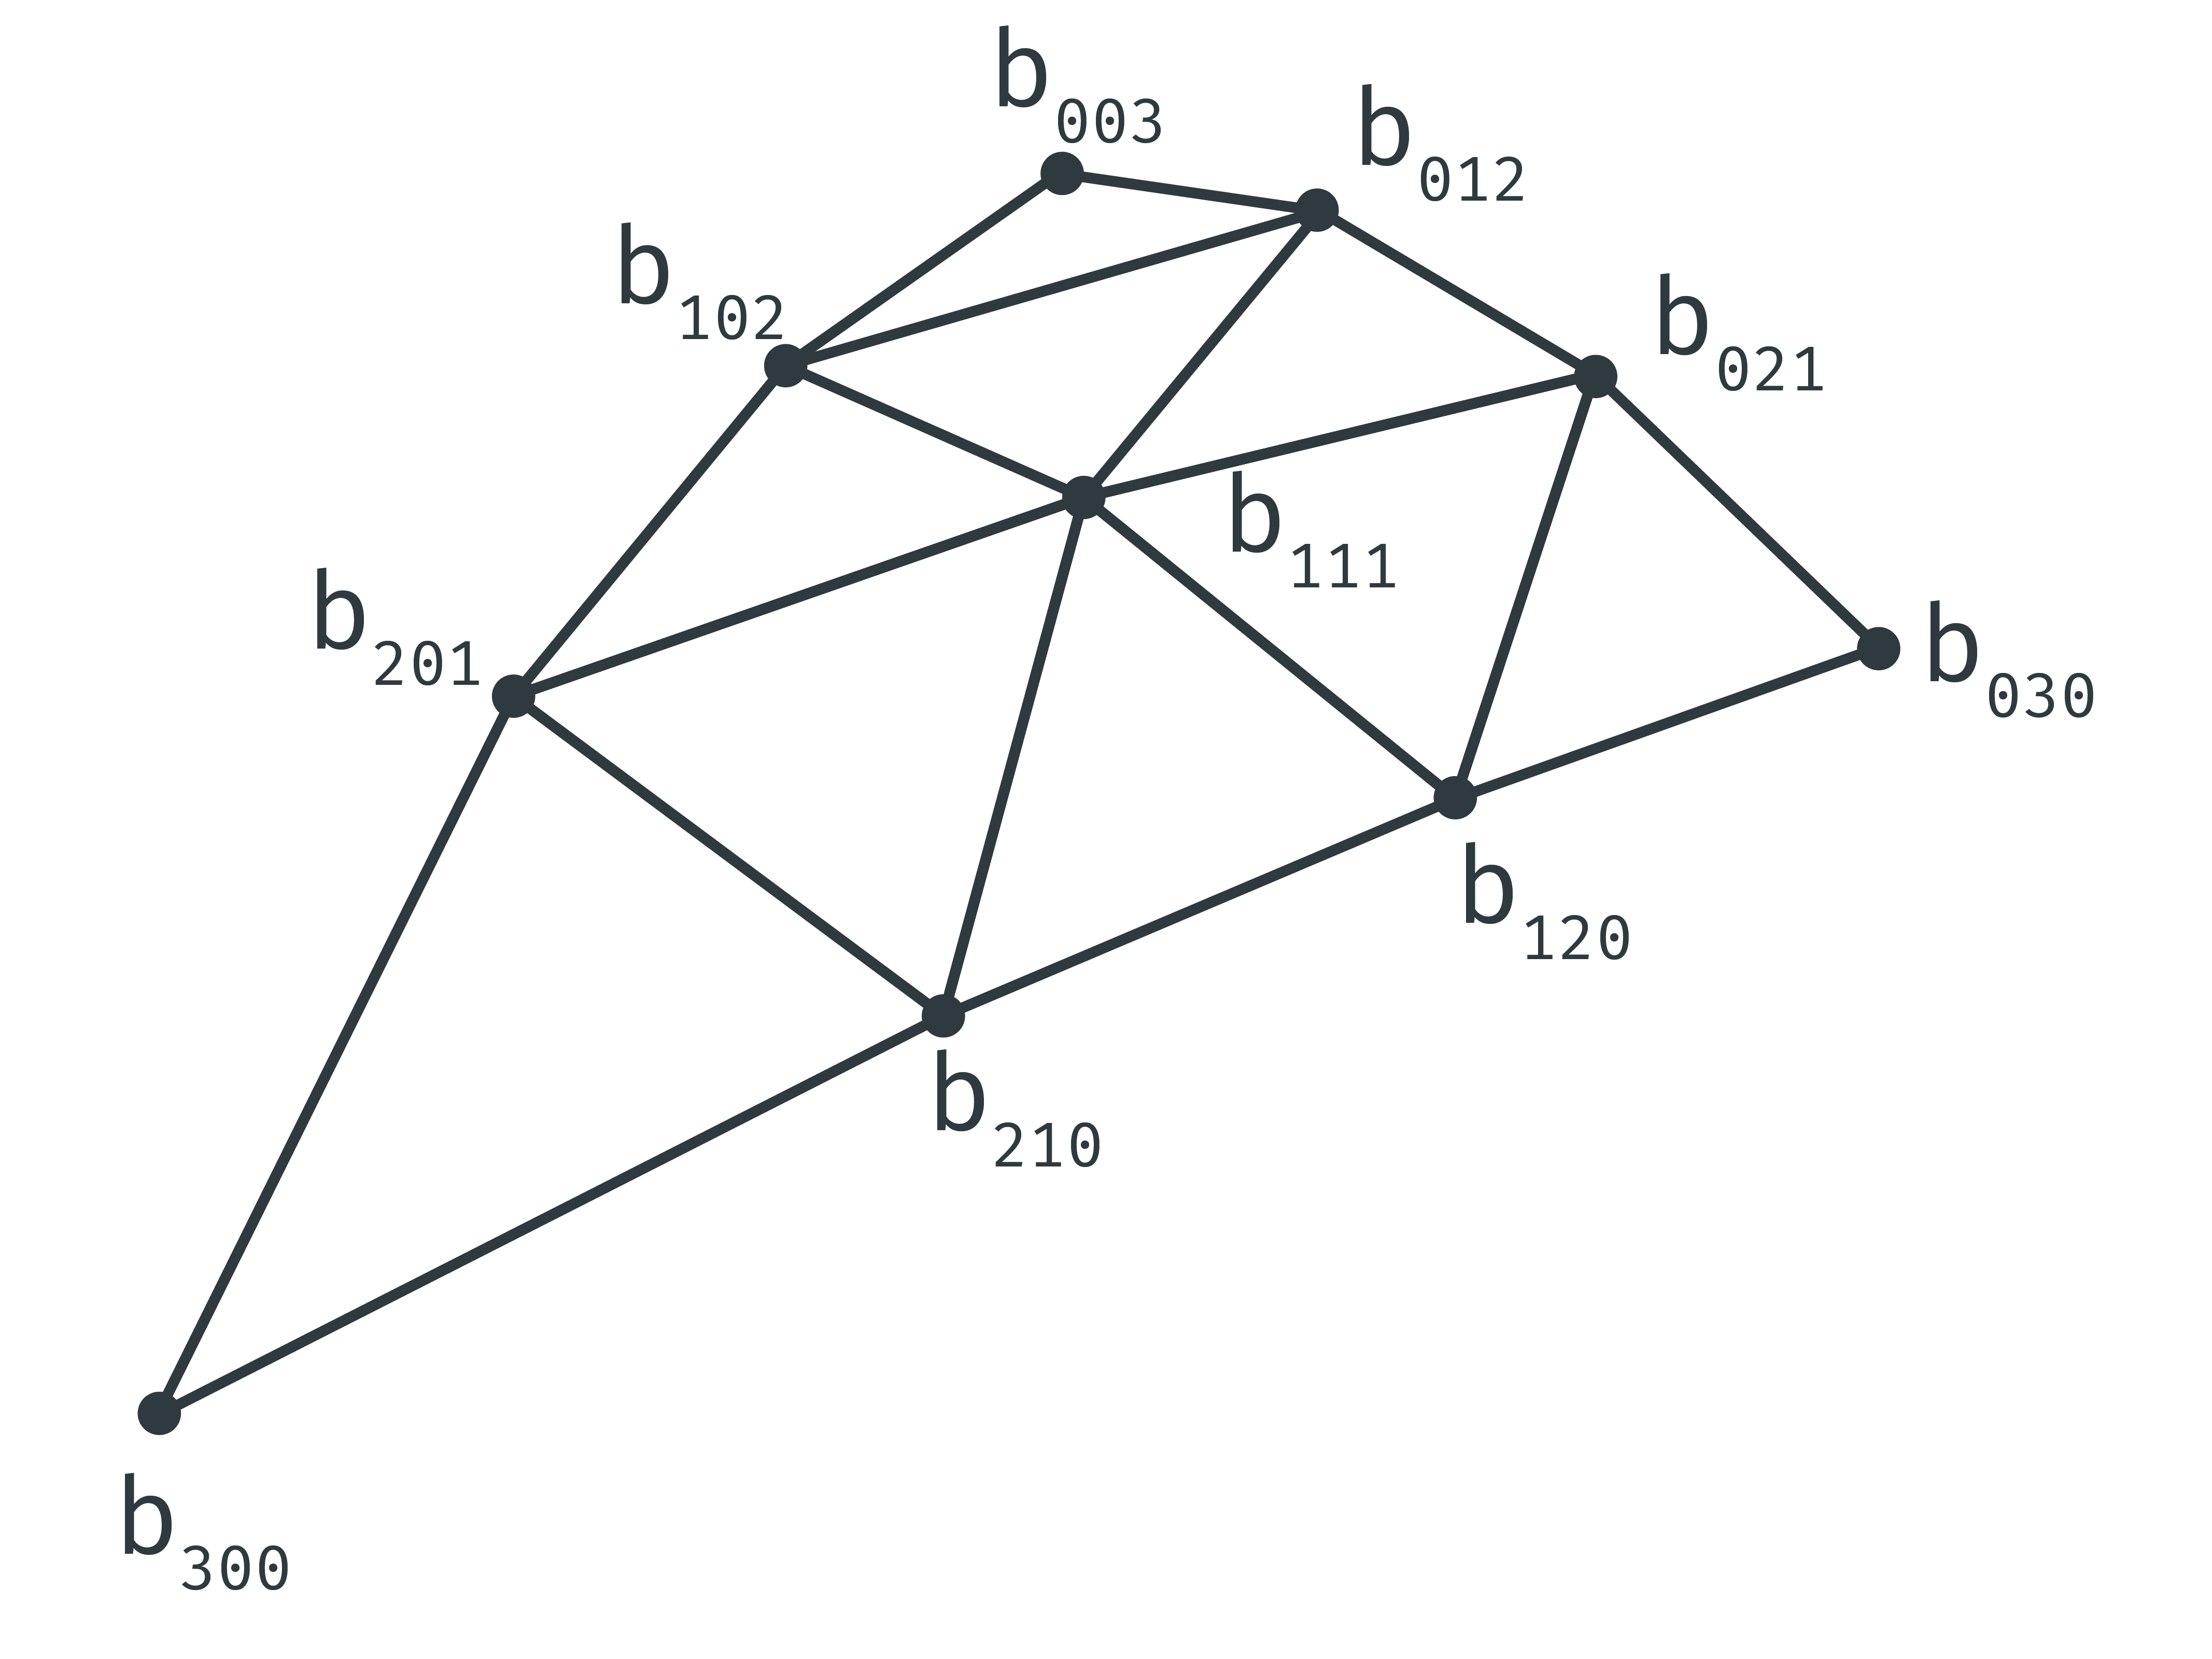
\includegraphics[width=0.45\textwidth]{./content/img/method/geometry.png}
	\caption{The geometric component of a point-normal triangle, i.e. the control net of a cubic Bézier triangle.}
	\label{fig:method:control_net}
\end{figure}
%
% ## Geometric component defined by triangluar cubic Bezier patch.
%
In the next subsection we discuss the definition of the geometry of a point-normal triangle. In subsection \crefs{sss:control_point_construction} we discuss the construction of the control points that define the geometry. 

\subsubsection{Basic form}
The geometric component of a point-normal triangle is defined as a triangular cubic Bézier patch. Such a patch $b(u,v)$ is defined as follows:
%
\begin{align}
\noalign{$b(u,v): \quad R^2 \mapsto R^3,\quad$ for $w = 1 - u - v, \quad u, v, w \geq 0$}
\begin{split}\label{eq:method:cubic_bezier_patch}
    b(u,v) ={}& \sum_{i + j + k = 3} b_{ijk}\frac{3!}{i!j!k!} u^i v^j w^k\\
      	   ={}& b_{300}w^3 + b_{030}u^3 + b_{003}v^3\\
      	    {}& + b_{210}3w^3 + b_{120}3wu^2 + b_{201}3w^2v\\
      	    {}& + b_{021}3u^2v + b_{102}2wv^2 + b_{012}3uv^2\\
      	    {}& + b_{111}6wuv.
\end{split}
\end{align}
%
The $b_{ijk}$ parameters in equation \ref{eq:method:cubic_bezier_patch} are the control points of the patch, also called coefficients. In \cref{fig:method:control_net} the visualization of the network of these control points is shown. We group the coefficients in three different groups, as their construction differs:
%
\begin{align*}
	\text{vertex coefficients: } {}&  b_{300},\ b_{030},\ b_{003} \\
	\text{tangent coefficients: } {}&  b_{210},\ b_{120},\ b_{021},\ b_{012},\ b_{102},\ b_{201}\\
	\text{center coefficient: }   {}&  b_{111}\\
\end{align*}

The formula in \eqref{eq:method:cubic_bezier_patch} can be used to evaluate any point parameterized by the barycentric coordinates $(u,v,w)$, on the patch. This is used in the sub-triangulation stage of the rendering process. In this stage the cubic Bézier surface is approximated by using a number of smaller flat triangles; these flat triangles are the triangles that are actually rendered. The number of sub-triangles is determined by the level of detail (lod). For the original sub-triangulation we refer the reader to \textcite{vlachos2001curved}, as this is where the implementation presented here deviates from the original. Details about this are provided in \crefs{s:implementation}.

As stated above the definition of the geometry of a point-normal triangle is a cubic Bézier patch. This degree of patches is a trade-off between simplicity, visual performance, and computational cost. Quadratic patches do not provide the same modeling range of a surface as a cubic patch, \citeauthor{boubekeur2008phong} \cite{boubekeur2008phong}. For example, a cubic representation is necessary to capture inflections implied by the triangle position and normal data. \citeauthor{vlachos2001curved} state that there is no additional data to suggest a higher degree is needed, and that therefore they settled on the form of $b(u,v)$ as presented in \crefe{eq:method:cubic_bezier_patch}.

\subsubsection{Coefficients} \label{sss:control_point_construction}
This section discusses how the `curved' control net geometry, (see \cref{fig:method:control_net}) is calculated from the flat input primitive shown in \cref{fig:method:input_primitive}. The input primitive provides the positions $P_1, P_2, P_3 \in \Real^3$ and normals $N_1, N_2, N_3 \in \Real^3$. The coefficients $b_{ijk}$ are computed as follows:
%
\begin{enumerate}[label=(\roman*)]
	\item 
		Initially, the coefficients $b_{ijk}$ are spread uniformly, i.e., the intermediate position of $b_{ijk}$ is calculated using the formula $(i P_i + j P_2 + kP_3) / 3$. 
	\item 
		The intermediate positions of the vertex coefficients are the same as their final positions, see equation \eqref{eq:method:vertex_coefficients}. Their intermediate position places them at the vertices of the input triangle, and this is where they are required to stay to keep the mesh watertight.
	\item 
		The tangent coefficients are placed at their final position by projecting the intermediate position into the tangent plane of the closest corner, see equation \eqref{eq:method:tangent_coefficients}. This is illustrated in \cref{fig:method:geometry_tangent_projection.png}.
	\item The center coefficient is moved to the average of the tangent coefficients plus $1/2$ times the distance it had to travel from its intermediate position, see equation \eqref{eq:method:center_coefficient}.
\end{enumerate}
%
\begin{figure}
	\centering
	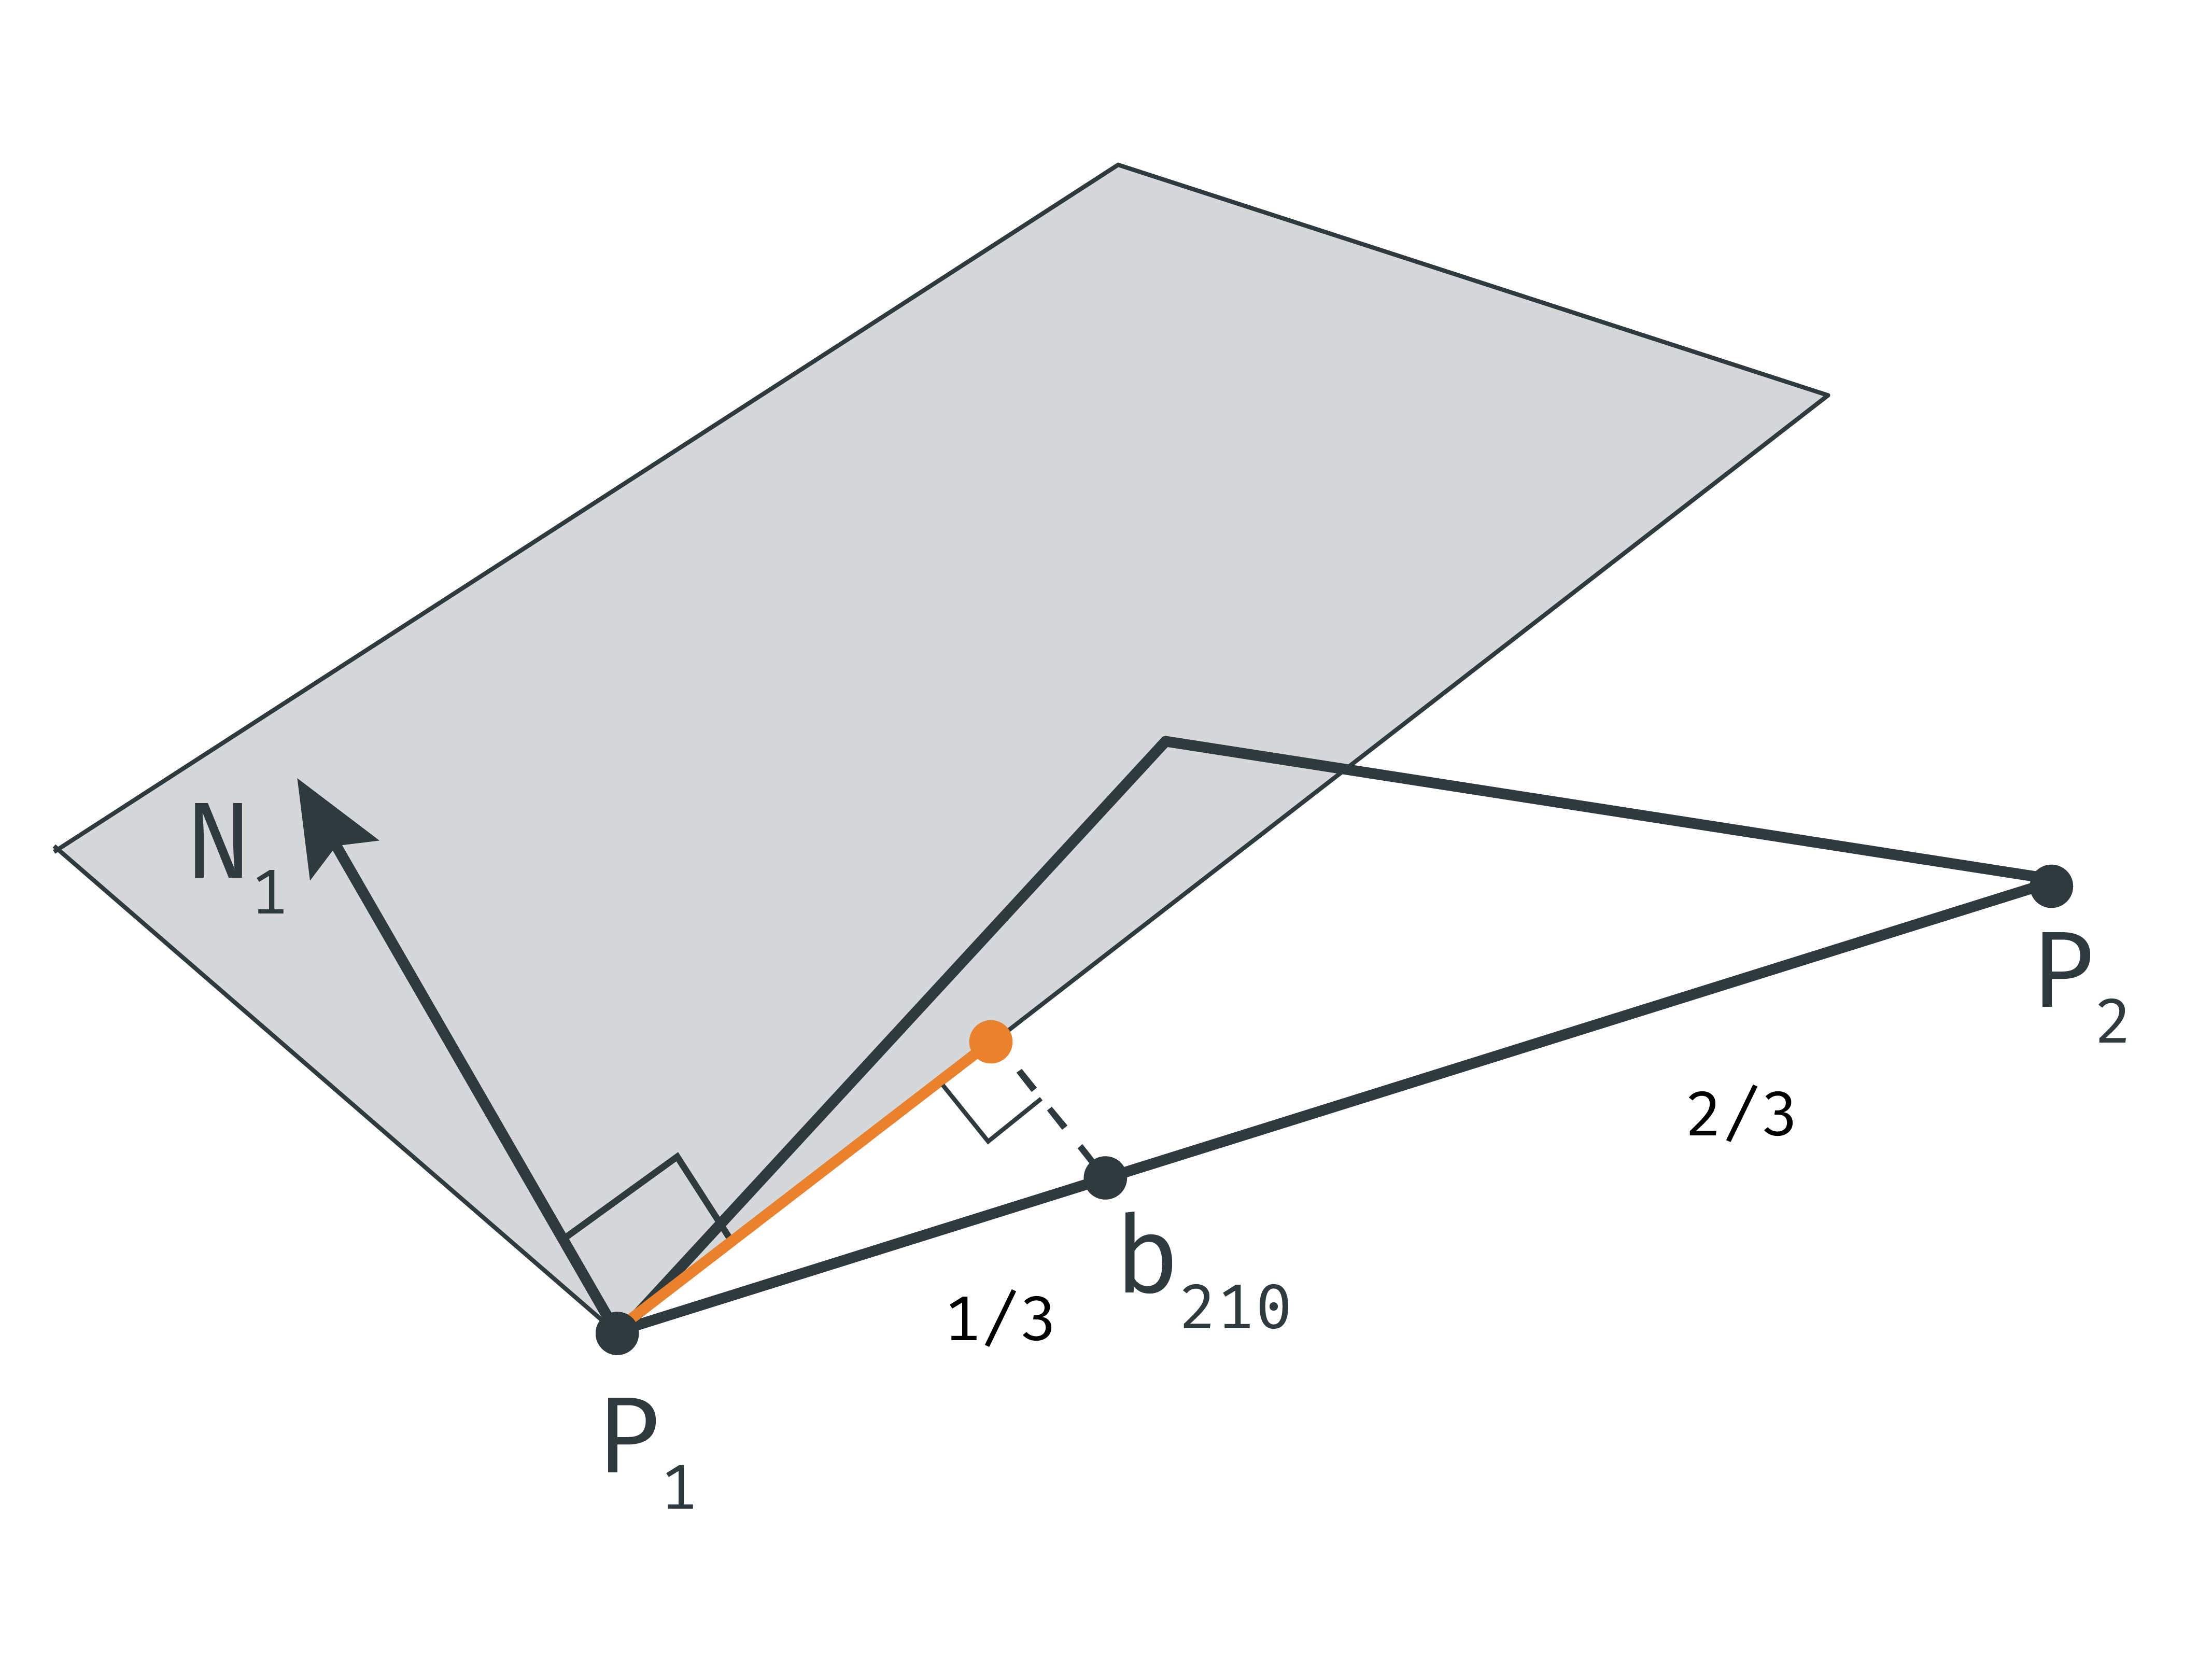
\includegraphics[width=0.45\textwidth]{./content/img/method/geometry_tangent_projection.png}
	\caption{Projection of a tangent coefficient $b_{210}$ to the tangent plane of the closes corner $P_1$.}
	\label{fig:method:geometry_tangent_projection.png}
\end{figure}


The following set of formulas describe how the positions of the coefficients are calculated. For clarity, we group together the formulas in the same way as the coefficients. This gives the following formulas for the \textit{vertex coefficients}:
\begin{align}\label{eq:method:vertex_coefficients}
	b_{300} = P_1,\ b_{030} = P_2,\ b_{003} = P_3.
\end{align}

The tangent coefficients are given by the projection of a point $Q$ onto the plane defined by the normal $N$ of the point $P$. The projected point $Q'$ is then given by: $Q' = Q - wN$, where $w = (Q - P) \cdot N$. Using this, the following set of formulas give the positions of the \textit{tangent coefficients}:
\begin{align}\label{eq:method:tangent_coefficients}
	w_{ij} = {}& (P_j - P_i) \cdot N_i \in \Real \nonumber\\
	b_{210} = {}& (2 P_1 + P_2 - w_{12}N_1) / 3,\nonumber\\
	b_{120} = {}& (2 P_2 + P_1 - w_{21}N_2) / 3,\nonumber\\
	b_{021} = {}& (2 P_2 + P_3 - w_{23}N_2) / 3, \\
	b_{012} = {}& (2 P_3 + P_2 - w_{32}N_3) / 3,\nonumber\\
	b_{102} = {}& (2 P_3 + P_1 - w_{31}N_3) / 3,\nonumber\\
	b_{201} = {}& (2 P_1 + P_3 - w_{13}N_1) / 3. \nonumber
\end{align}

The last coefficient is the center coefficient which is, as stated before, moved to the average of the previous computed tangent coefficients plus $1/2$ times the distance it traveled from its intermediate location to that average position. The \textit{center coefficient}, is computed by:
\begin{align}\label{eq:method:center_coefficient}
	E = {}& (b_{210} + b_{120} + b_{021} \nonumber \\
		{}& + b_{012} + b_{102} + b_{201}) / 6, \nonumber\\
	V = {}& (P_1 + P_2 + P_3) / 3, \\
	b_{111} = {}& E + (E - V) / 2. \nonumber
\end{align}
Combining \eqref{eq:method:vertex_coefficients} through \eqref{eq:method:center_coefficient} transforms the input primitive (see \cref{fig:method:input_primitive}) to the control net shown in \cref{fig:method:control_net}.


\subsubsection{Properties}
\label{sss:method:geometric:properties}
\citeauthor{vlachos2001curved} have shown that point-normal triangles do not deviate too much from the original triangle. This is an important property since this ensures that the shape of the model is preserved and adjacent triangles do not interfere with each other. 

By demanding shared normals, i.e., one unique normal per vertex, the boundary between two point-normal triangles is generated by the same algorithm, thus the surface is water tight. Except at the corners, PN triangles do not usually join with tangent continuity \cite{vlachos2001curved}. \Cref{fig:method:cracks} illustrates what happens if normals are not shared.

\begin{figure}
	\ooit{Moeten dit plaatje eigenlijk maken met driehoeken.}
	\centering
	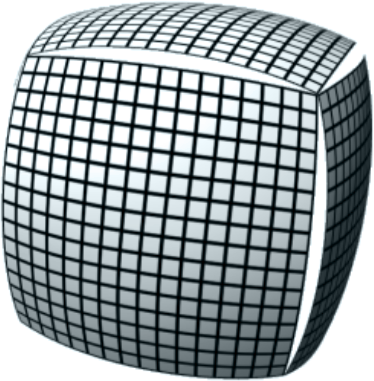
\includegraphics[width=0.4\columnwidth]{./content/img/method/cracks.png}
	\caption{Illustration of what would happen if one renders a model using point-normal triangles where vertices have different normals, depending on the associated faces. Image taken from \cite{mcdonald2010crack}.}
	\label{fig:method:cracks}
\end{figure}

%!TEX root = ../main.tex

\subsection{Normal component}\label{ss:normal_component}
% What?
This section discusses the parametrization of both the `fake' and `real' normals. We differentiate between these two normal types because originally point-normal triangles normals are interpolated based on a quadratic patch, the `fake' normals (see \crefs{sss:method:normals:fakeNormals}), whereas one would get the `real' normals by calculating them based on the actual surface (see \crefs{sss:method:normals:realNormals}).

It should be noted that, just as with the geometric component, the normal component of the point-normal triangle is computed solely based on the input primitive, i.e., the vertex positions and their normals, as shown in \cref{fig:method:input_primitive}. 

\begin{figure}
	\centering
	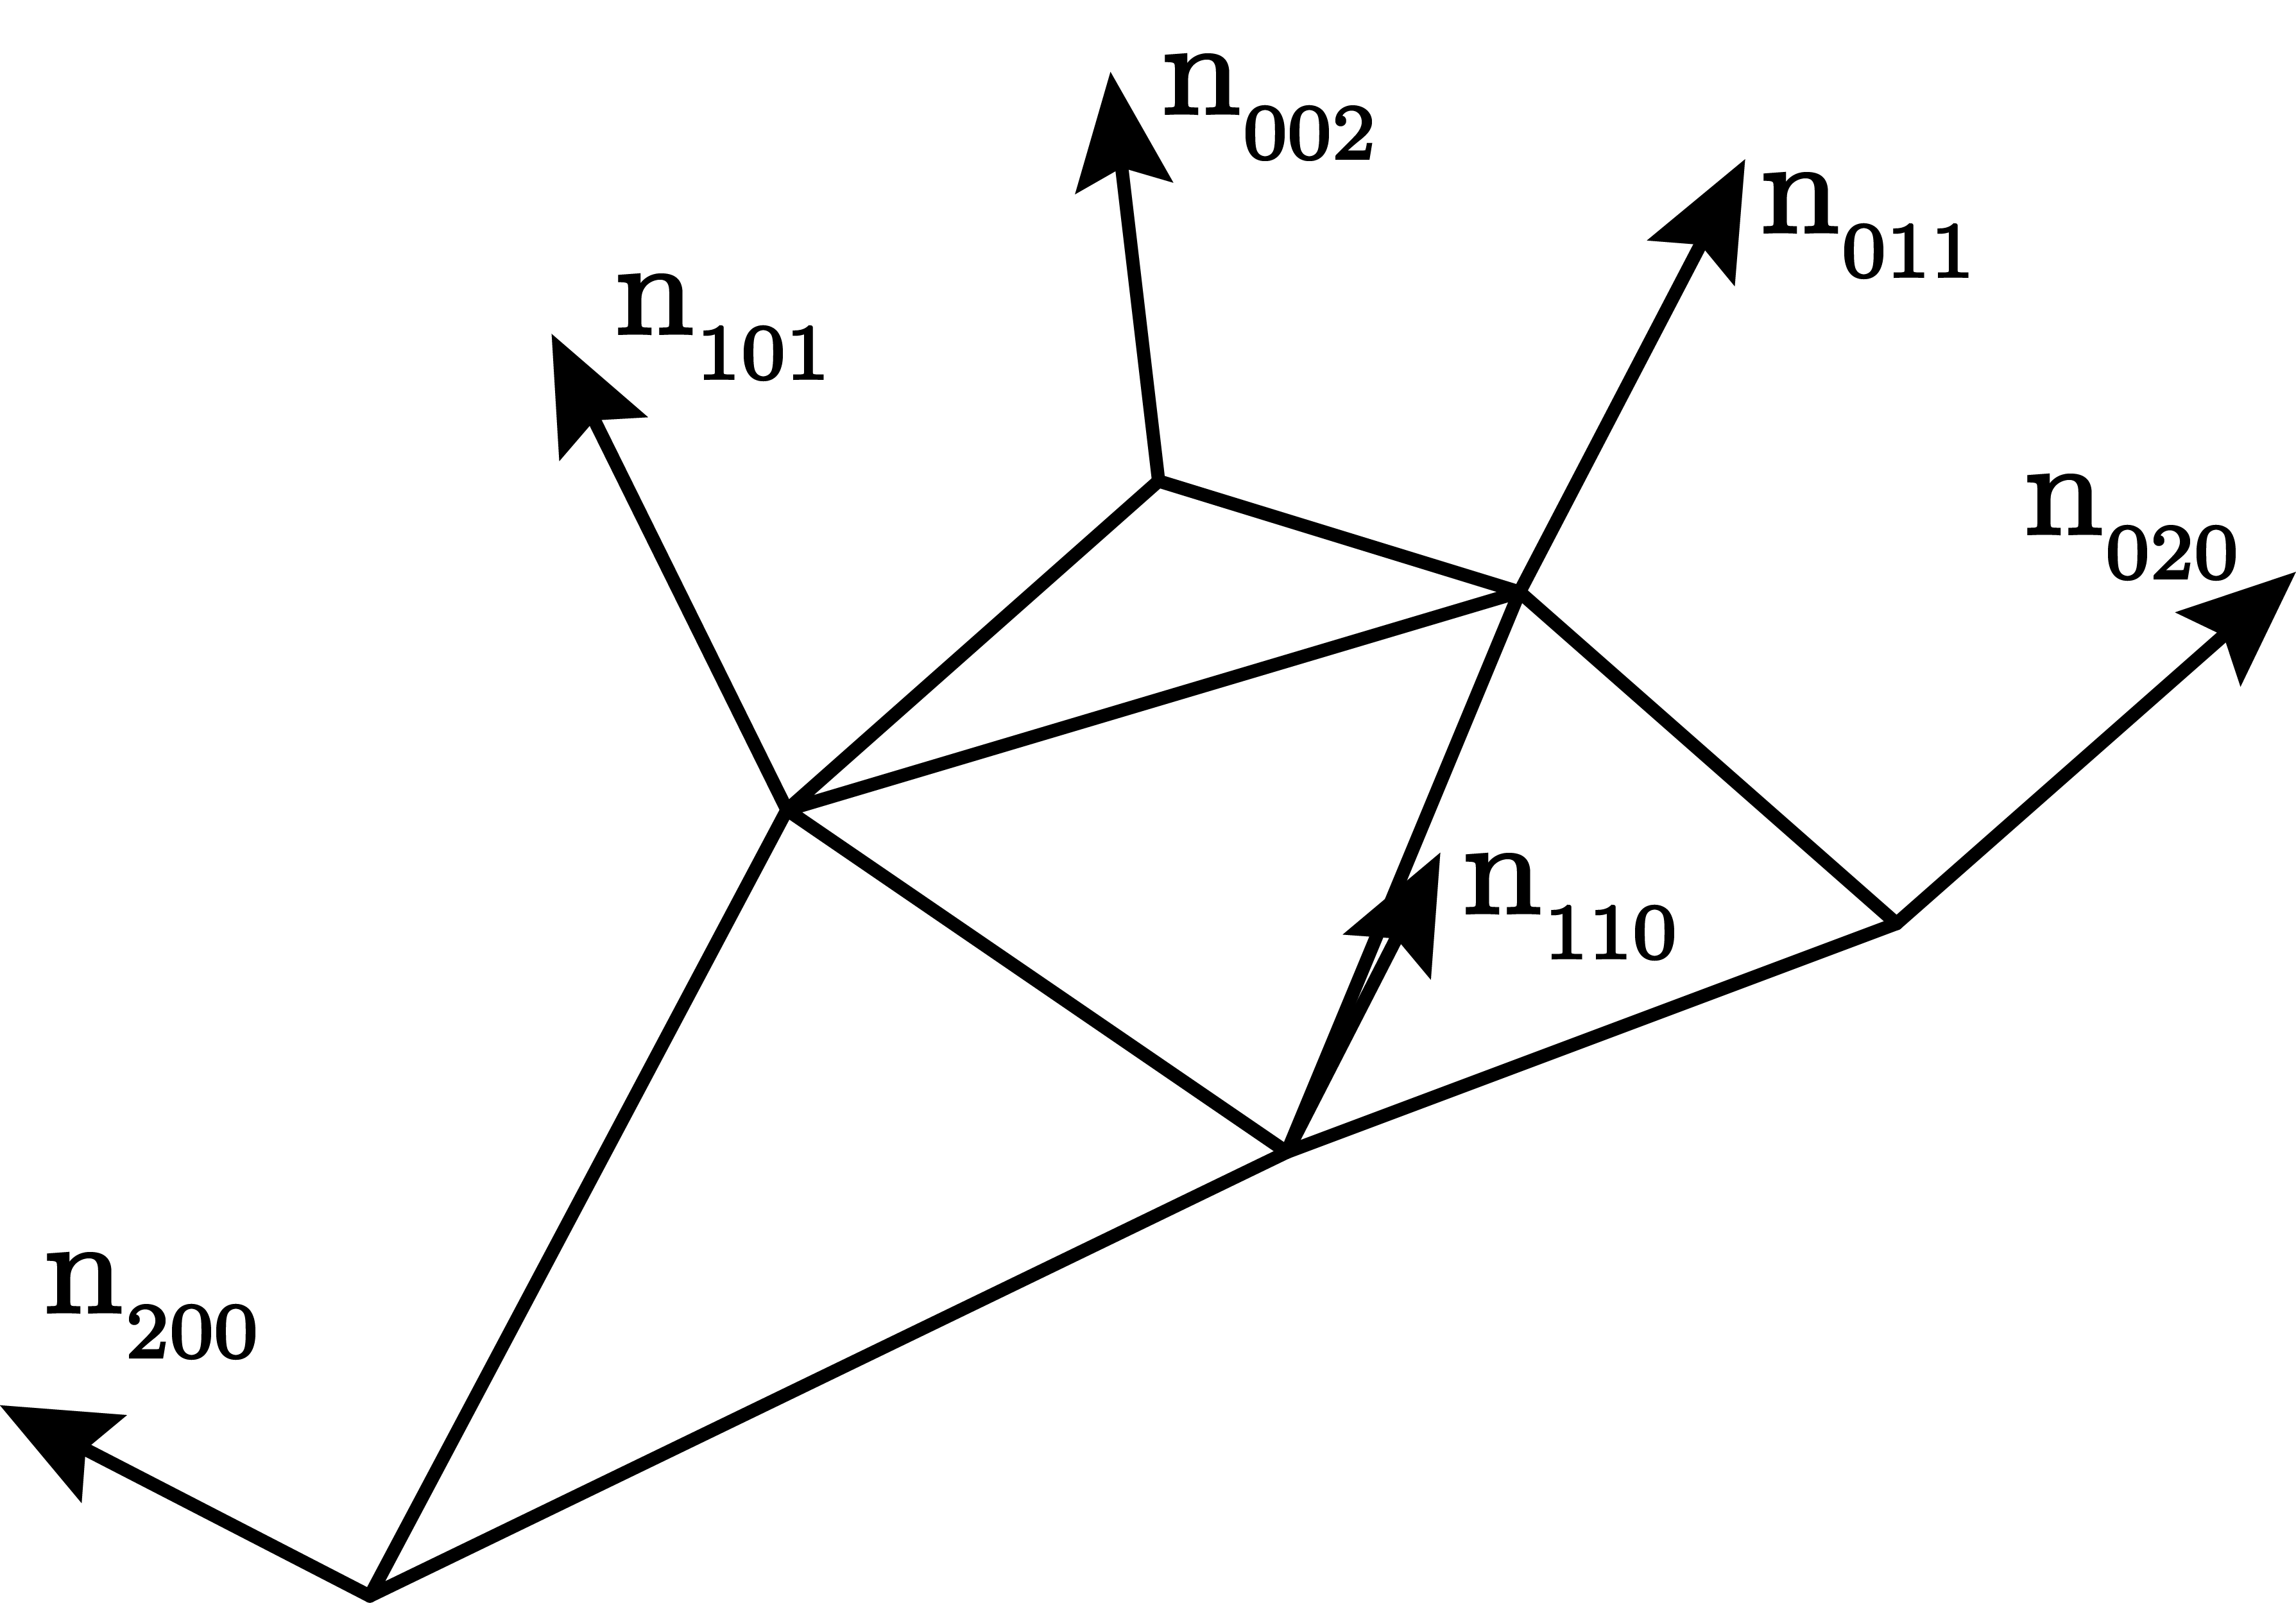
\includegraphics[width=0.45\textwidth]{./content/img/method/normals.png}
	\caption{The normal field of the point-normal triangle.}
	\label{fig:method:normal_field}
\end{figure}

\subsubsection{Fake normals}
\label{sss:method:normals:fakeNormals}
	\citeauthor{vlachos2001curved} define the `fake' normals using a quadratic function $n(u,v)$:
	\begin{align}
	\noalign{$n(u,v): \quad R^2 \mapsto R^3,\quad$ for $w = 1 - u - v, \quad u, v, w \geq 0$}
	\begin{split}\label{eq:method:quadratic_normal_patch}
	    n(u,v) ={}& \sum_{i + j + k = 2} n_{ijk}u^i v^j w^k,\\
	      	   ={}& n_{200}w^2 + n_{020}u^2 + n_{002}v^2\\
	      	    {}& + n_{110}wu + n_{011}uv + n_{101}wv\\
	\end{split}
	\end{align}
	The coefficients of this quadratic `patch' are the normals shown in \cref{fig:method:normal_field}. The normals are computed for a point, halfway on every edge, i.e., $(u,v,w) = (\frac{1}{2}, \frac{1}{2}, 0)$, $(0, \frac{1}{2}, \frac{1}{2})$, $(\frac{1}{2}, 0, \frac{1}{2})$. Point-normal triangles use quadratically varying normals to be able to capture the inflection points that are possible due to the cubic geometric component. 

	\Cref{fig:method:linear_vs_quadratically_varying} illustrates why one needs quadratic patches to capture these inflection points. \Cref{fig:method:linear_vs_quadratically_varying} illustrates two cases: \cref{fig:method:normal:both} shows that when the normals point in a different direction the surface will be parabolic, and no inflection point exists. In this case both linear and quadratically varying normals are able to capture the surface. In \cref{fig:method:normal:linear} and \cref{fig:method:normal:quadratic} the case were an inflection point exists is shown. We see that (\cref{fig:method:normal:linear}) linear varying normals do not capture the inflection point, i.e., give incorrect normals. The quadratically varying normals do give the correct normals (\cref{fig:method:normal:quadratic}), i.e, they capture the inflection point.

	\begin{figure}
		\centering
		\begin{subfigure}{\columnwidth}
			\centering
			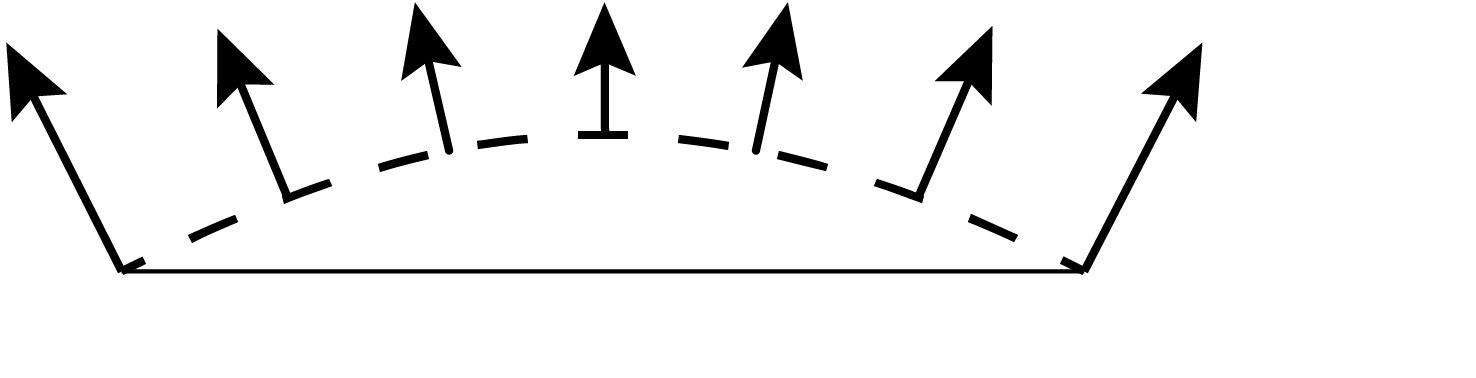
\includegraphics[width=0.8\textwidth]{./content/img/method/linearVsQuadraticNormals_both.png}
			\caption{Vector averaging with either linear or quadratic over a curve without inflections.}
			\label{fig:method:normal:both}
		\end{subfigure}
		\begin{subfigure}{\columnwidth}
			\centering
			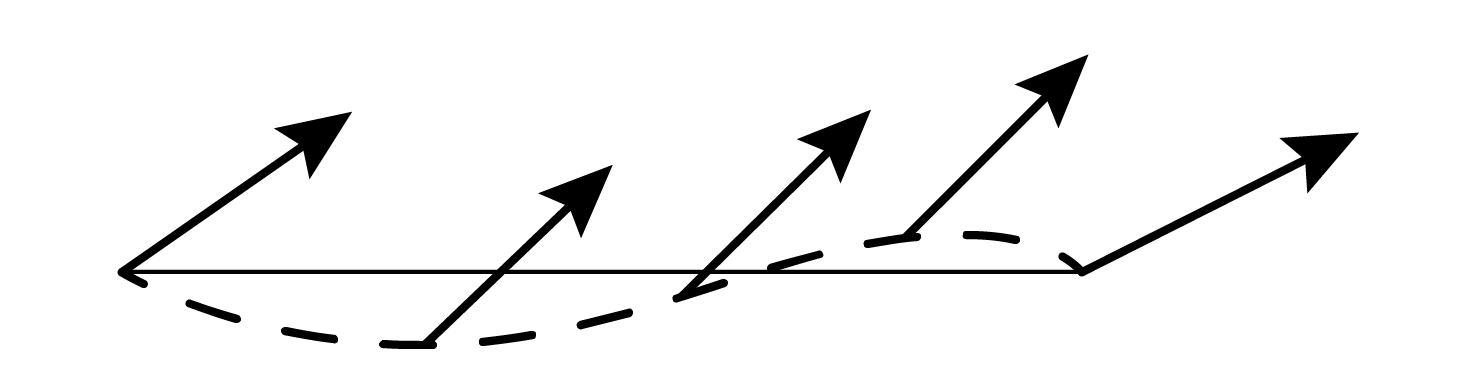
\includegraphics[width=0.8\textwidth]{./content/img/method/linearVsQuadraticNormals_linear}
			\caption{Vector averaging with linear interpolation over a curve with an inflection.}
			\label{fig:method:normal:linear}
		\end{subfigure}	
		\begin{subfigure}{\columnwidth}
			\centering
			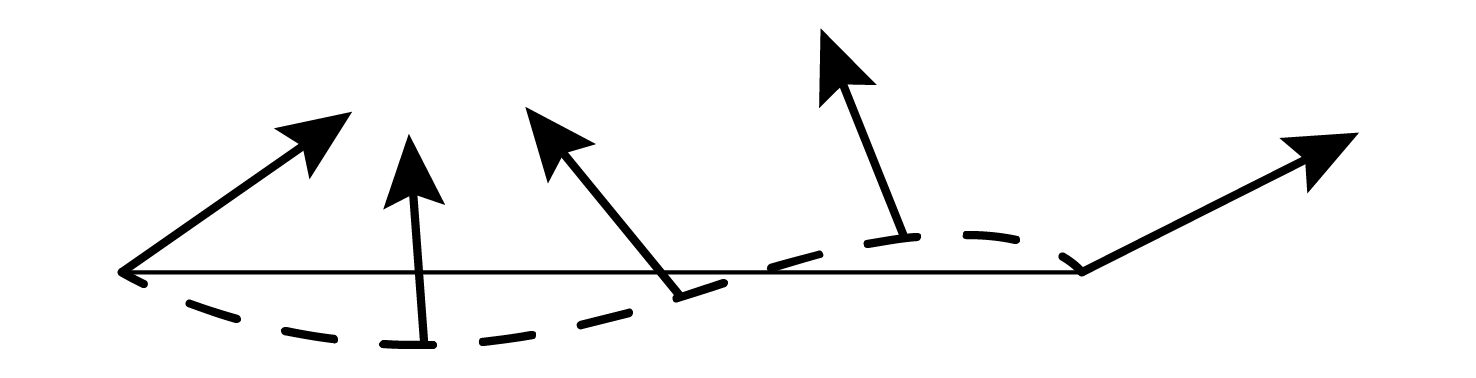
\includegraphics[width=0.8\textwidth]{./content/img/method/linearVsQuadraticNormals_quadratic}
			\caption{Vector averaging with quadratic interpolation over a curve with an inflection.}
			\label{fig:method:normal:quadratic}
		\end{subfigure}			
		\caption{Examples of normal vector averaging over an edge. The dashed lines indicate the profile of the surface that should be approximated. The normals of a curves without inflections are correctly approximated by both linear and quadratic interpolation, see \cref{fig:method:normal:both}. The normals of a curve with inflections are incorrectly approximated with \subref{fig:method:normal:linear} linear interpolation and correctly with \subref{fig:method:normal:quadratic} interpolation. Image \subref{fig:method:normal:both} was adapted from \cite{van1997phong}, image \subref{fig:method:normal:linear} and \subref{fig:method:normal:quadratic} from \cite{vlachos2001curved}.}
		\label{fig:method:linear_vs_quadratically_varying}
	\end{figure}

	\todo[inline]{Discuss parametrization of `quadratic' patch}

	Using the function $n(u,v)$, see \eqref{eq:method:quadratic_normal_patch}, the normal of any point parametrized by the barycentric coordinates $(u,v)$ can be calculated. To do this we first need to define a control net. We consider two different types of coefficients: the vertex normals, $n_{200}$, $n_{020}$, and $n_{002}$; and the edge normals, $n_{110}$, $n_{011}$, and $n_{101}$.
	\todo[inline]{Discuss the construction of the control points for the `quadratic' patch}

	An edge normal is calculated by taking the average of the two input vertex normals of the vertices of the edge. After this step this looks like the image shown in \cref{fig:method:normal:linear}. To capture the inflection point the average normal is then reflected across the plane perpendicular to the edge, see \cref{fig:method:normal:reflection}. When a inflection point exists this will give the correct mid-edge normal (see \cref{fig:method:normal:quadratic}) and this will also not alter the normal field if no inflection point is present, e.g., imagine reflecting the mid-edge normal of the curve shown in \cref{fig:method:normal:both}, this will result in the same normals.

	\begin{figure}
		\centering
		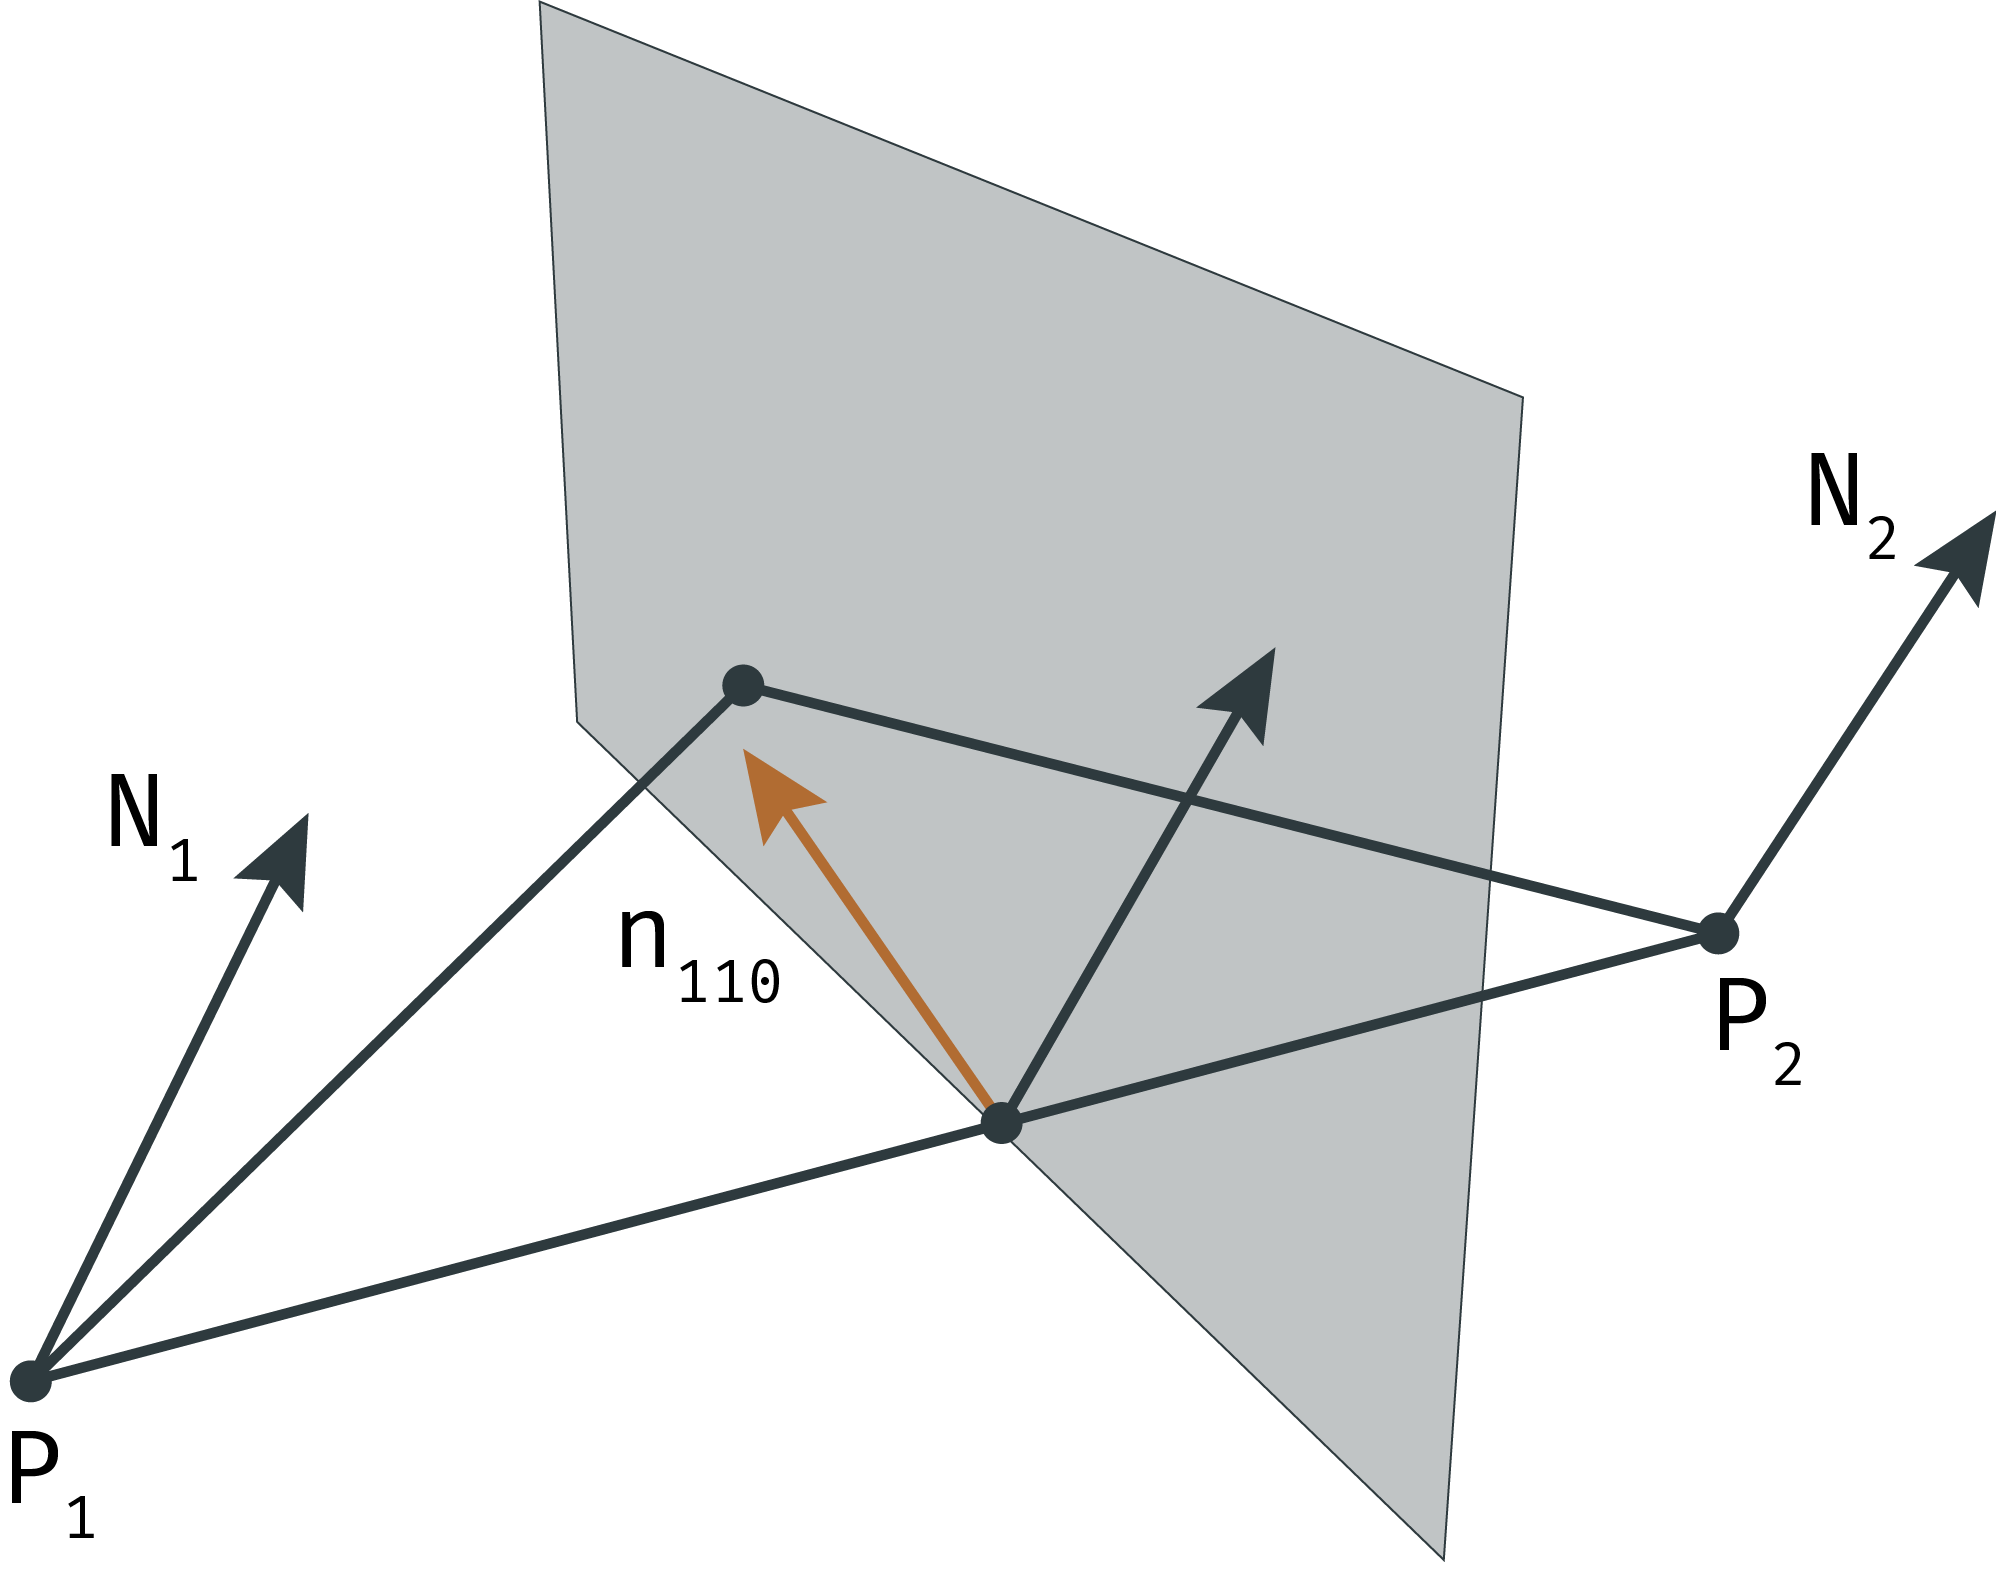
\includegraphics[width=0.45\textwidth]{./content/img/method/normal_reflection.png}
		\caption{Construction of the mid-edge normal coefficient, used for quadratically varying normals. The two input normals are averaged and then reflected reflected across the plane perpendicular to the edge.}
		\label{fig:method:normal:reflection}
	\end{figure}

	The vertex normals are simply the normals provided by the input primitive.

\subsubsection{Real normals}
\label{sss:method:normals:realNormals}
		\todo[inline]{Discuss how to compute the real normals given the geometric component}
		The real normals are computed based on the geometric component of the point-normal triangle. This is done by taking the cross product of the the partial derivatives with respect to $u$ and $v$. For the partial derivatives with respect to $u$ and $v$ see \eqref{eq:method:normal:partialU} and \eqref{eq:method:normal:partialV} respectively.

		\begin{align} \label{eq:method:normal:partialU}
			\frac{\partial b(u,v)}{\partial u} ={}& \sum_{i + j + k = 2} b_{i+1, j, k} \frac{2!}{i!j!k!} u^i v^j w^k  \nonumber\\
										   ={}& w^2 b_{102} + v^2 b_{120} + u^2 b_{300} + \\
										    {}& 2 v w b_{111} + 2 u w b_{201} + 2 u v b_{210} \nonumber 
		\end{align}

		\begin{align} \label{eq:method:normal:partialV}
			\frac{\partial b(u,v)}{\partial v} ={}& \sum_{i + j + k = 2} b_{i, j + 1, k} \frac{2!}{i!j!k!}u^i v^j w^k \nonumber \\
											   ={}& w^2 b_{012} + v^2 b_{030} + u^2 b_{210} + \\
											    {}& 2 v w b_{021} + 2 u w b_{111} + 2 u v b_{120} \nonumber
		\end{align}

		The partial derivatives in \eqref{eq:method:normal:partialU} and \eqref{eq:method:normal:partialV} define two tangent vectors in the $u$ and $v$ directions, at a point $(u,v)$ of the surface. By taking the crossproduct of these two vectors, at a point, we find the `real' normal of that point defined by the geometric component of the point-normal triangle.


%!TEX root = ../main.tex

\section{Implementation}
\label{s:implementation}
\rick{Nalezen:}

\begin{figure}
	\plaatje{Pas de kleuren aan, pas het font aan, maak de pipelines verticaal, laat de twee teseelations shaders zien, geef alle blokjes dezelfde stijl, met tikz maken?}
	\centering
	\begin{subfigure}{\columnwidth}
		\centering
		
\includegraphics[width=\columnwidth]{content/img/implementation/pipeLineOld.png}
		\caption{The graphics pipeline of OpenGL version 1.3 (2001).}
		\label{fig:implementation:pipeline:old}
	\end{subfigure}
	\begin{subfigure}{\columnwidth}
		\centering
		
\includegraphics[width=\columnwidth]{content/img/implementation/pipeLineNew.png}
		\caption{The graphics pipeline of OpenGL version 4.1 (2010).}
		\label{fig:implementation:pipeline:new}
	\end{subfigure}	
	\caption{A schematic overview of the programmable parts of the \subref{fig:implementation:pipeline:old} 1.3 and \subref{fig:implementation:pipeline:new} 4.1 OpenGL graphics pipelines. Each rounded rectangle represents one programmable shader.}
	\label{fig:implementation:pipeline}
\end{figure}

A schematic overview of both the OpenGL pipeline at the time of the publication of the paper and the introduces PN-triangles and the current pipeline are presented in \cref{fig:implementation:pipeline}. These images show that since \citeyear{vlachos2001curved} three new shaders have been introduced into the pipeline, namely the tessellation control, tessellation evaluation and the geometry shader. 

Since only the tessellation shaders are relevant for point-normal triangles we discuss those in more detail in section \ref{ss:implementation:pipeline}. Section \ref{ss:implementation:tcs} through section \ref{ss:implementation:tes} present our implementation of point-normal triangles per discussed tessellation stage. 

\subsection{The OpenGL Pipeline}
\label{ss:implementation:pipeline}

	\begin{figure}
		\centering
		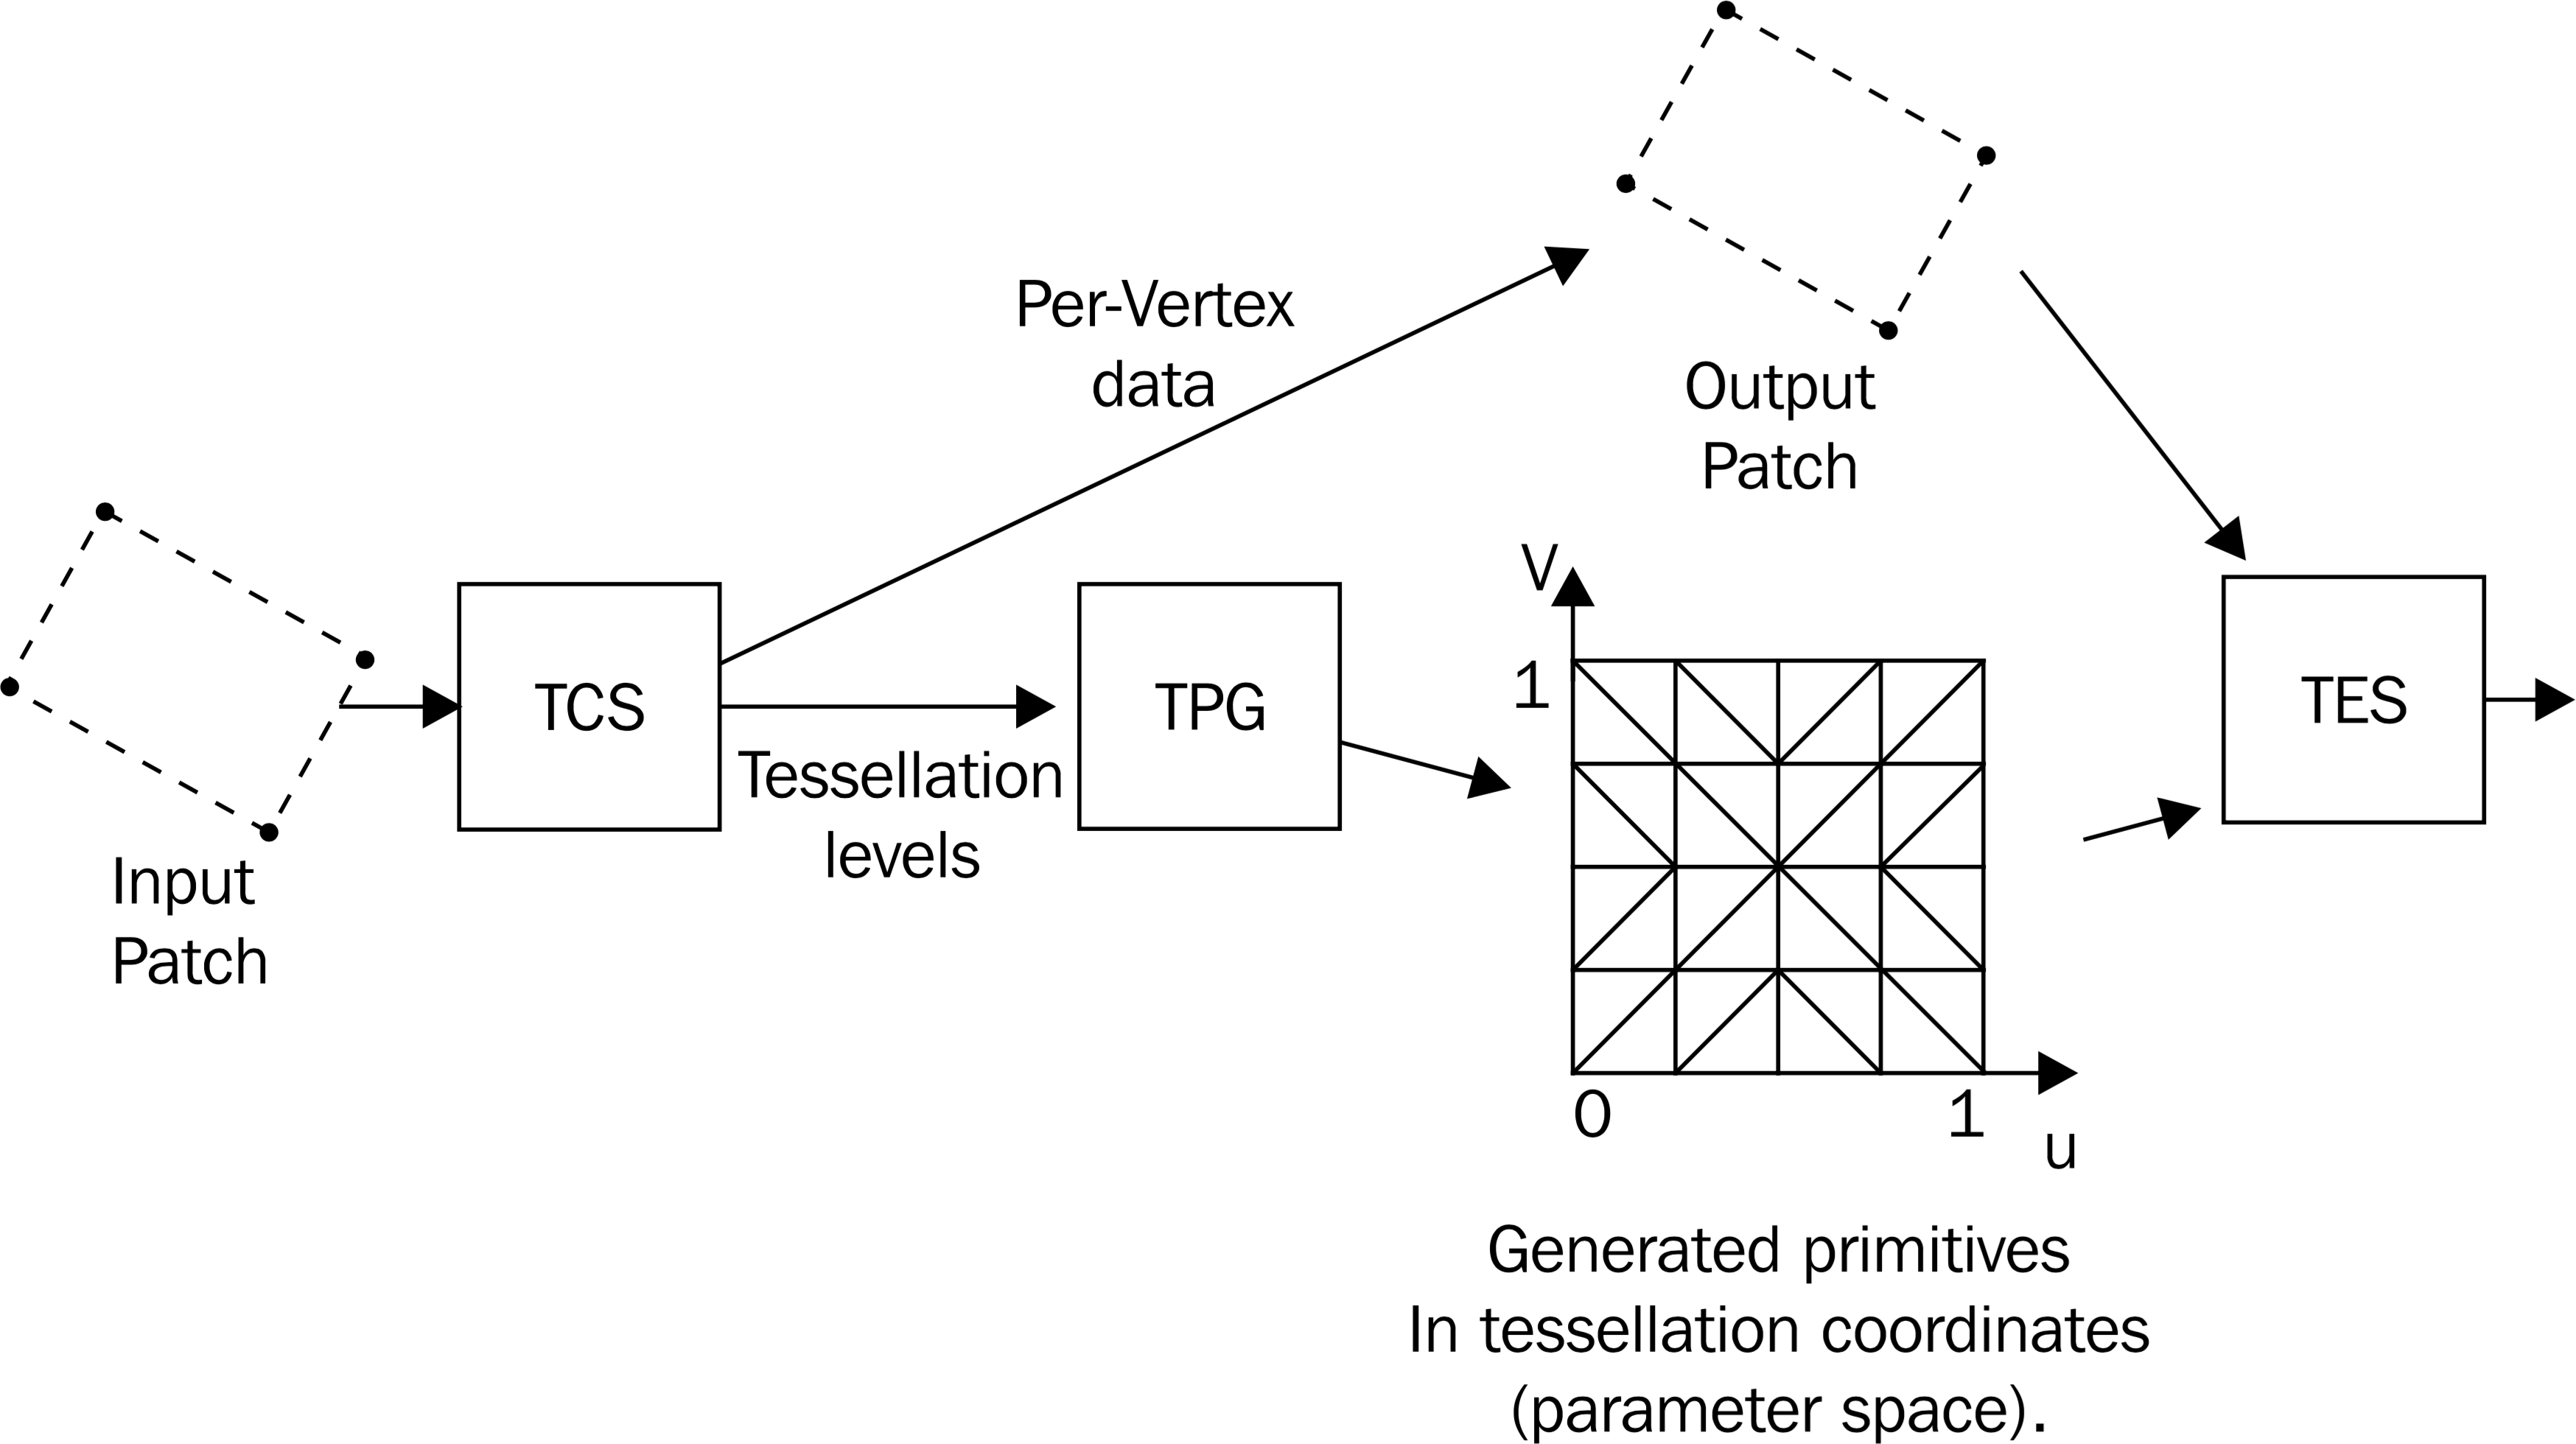
\includegraphics[width=\columnwidth]{content/img/implementation/tesselationPipeline.png}
		\caption{An overview of the tessellation part of the OpenGL render pipeline. Note that in the case of point-normal triangles the input patches, generated primitives and output patches are triangles, not quads. Illustration taken form \textcite{wolff2013opengl}.}
		\label{fig:implementation:tessellationPipeline}
	\end{figure}

	% Tesselation:
	A schematic overview of tessellation in OpenGL is presented \Cref{fig:implementation:tessellationPipeline}.
	% Tesselation control
	% Invoked for
	The tessellation control shader (TCS) is invoked once for each vertex in the output patch, a triangle in our case. 
	% What does it do
	The primary function of the tessellation control shader is the setting of both the inner and the outer tessellation levels. Additionally the TCS can compute additional information about the vertices in the input patch. 
	% Output:
	As can been seen in \cref{fig:implementation:tessellationPipeline} the TCS passes additional information about that patch along to the tessellation evaluation shader (TES) via the output patch. The tessellation levels are sent to the tessellation primitive generator (TPG) \cite{wolff2013opengl}.

	The TPG generates a number of new primitives based on the tessellation levels. How these primitives are generated depends on the selected edge tessellation spacing. Equal spacing results in evenly divided edges, whereas fractional spacing allows for two shorter edges in the subdivision for more stable interpolation under changing tessellation levels \cite{wolff2013opengl,openGL41Core}.

	% Tesselation evaluation
	% Invoked for
	The tessellation evaluation shader (TES) is executed for each vertex that is generated by the TPG. 
	% Input:
	It receives the coordinates of this vertex in parameter space and the output of the TCS, as is illustrated in \cref{fig:implementation:tessellationPipeline}. 
	% What does it do
	Based on this information it computes the position of the current vertex. 
	% Output:
	This shader is passed to the next shader in the pipeline, either the geometry shader or the fragment shader, see \cref{fig:implementation:pipeline:new}.

\subsection{Tesselation Control Shader}
\label{ss:implementation:tcs}
	% Geometry

	% Fake normals

	% Real normals

\subsection{Tessellation Primitive Generator}
\label{ss:implementation:tpg}
	% Geometry

	% Fake normals

	% Real normals

\subsection{Tessellation Evaluation Shader}
\label{ss:implementation:tes}
	% Geometry

	% Fake normals

	% Real normals

%!TEX root = ../main.tex

\section{Results}
\label{s:results}
In this section we present our results. \Crefs{s:results:normals} compares the computational complexity of the computation of the `real' and `fake' normals. Furthermore it contrasts the visual results. \Crefs{s:results:pipeline} contrasts the results of the implementation by \citeauthor{vlachos2001curved} on the CPU with our implementation on the GPU.

%!TEX root = ../main.tex
\subsection{Fake versus real normals}
\label{s:results:normals}
	\todo[inline]{Show results of PN triangles with fake and real normals, and discuss differences}
	\todo[inline]{Computational complexity of the fake normals and the real normals, consider one triangle.}
	\todo[inline]{Any unsolved problems?}

\iftoggle{PHONG}{
	\subsection{Phong tesselation versus PN triangles}
	\future{Show comparison of Phong tesselation with PN triangles: performance, visual results, continuity, probably in cooperation with Jelle and Gerben}
	\future{Any unsolved problems?}
}

%!TEX root = ../main.tex

\subsection{Pipeline}
\label{s:results:pipeline}
	\Cref{fig:results:cpugpu} shows the rendering by \citeauthor{vlachos2001curved} next to our rendering of, probably, the same model. The only difference between these two models should be the pattern in which the triangles of the input mesh are subdivided into flat triangles. A visual inspection shows no obvious differences between the models, leading us to suggest that the difference in triangulation does not matter much. 

	%!TEX root = ../main.tex
\begin{figure*}
	\centering
	\begin{subfigure}[b]{0.2\textwidth}
		\centering
		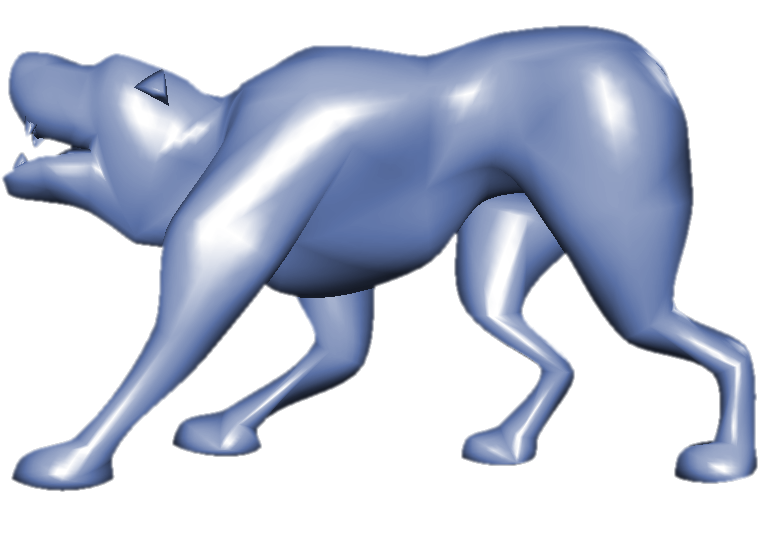
\includegraphics[width=\textwidth]{content/img/results/cpugpu/dogCPU.png}
		\caption{Rottweiler on CPU}
		\label{fig:results:cpugpu:cpuDog}
	\end{subfigure}
	\hspace{0.1\textwidth}
	\begin{subfigure}[b]{0.2\textwidth}
		\centering
		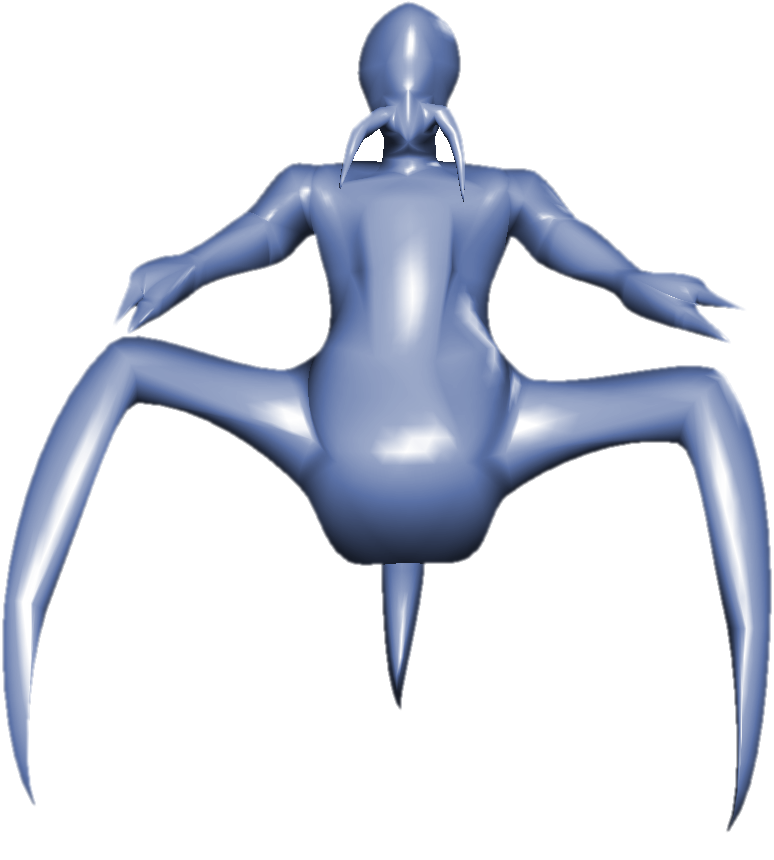
\includegraphics[width=\textwidth]{content/img/results/cpugpu/voreCPU.png}
		\caption{Vore on CPU}
		\label{fig:results:cpugpu:cpuVore}
	\end{subfigure}	
	\hspace{0.1\textwidth}
	\begin{subfigure}[b]{0.2\textwidth}
		\centering
		\includegraphics[width=\textwidth]{content/img/results/cpugpu/shamblercpu.png}
		\caption{Shambler on CPU}
		\label{fig:results:cpugpu:cpuShambler}
	\end{subfigure}		

	\begin{subfigure}[b]{0.2\textwidth}
		\centering
		\includegraphics[width=\textwidth]{content/img/results/cpugpu/doggpu.png}
		\caption{Rottweiler on GPU}
		\label{fig:results:cpugpu:gpuDog}
	\end{subfigure}
	\hspace{0.1\textwidth}
	\begin{subfigure}[b]{0.2\textwidth}
		\centering
		\includegraphics[width=\textwidth]{content/img/results/cpugpu/voregpu.png}
		\caption{Vore on GPU}
		\label{fig:results:cpugpu:gpuVore}
	\end{subfigure}	
	\hspace{0.1\textwidth}
	\begin{subfigure}[b]{0.2\textwidth}
		\centering
		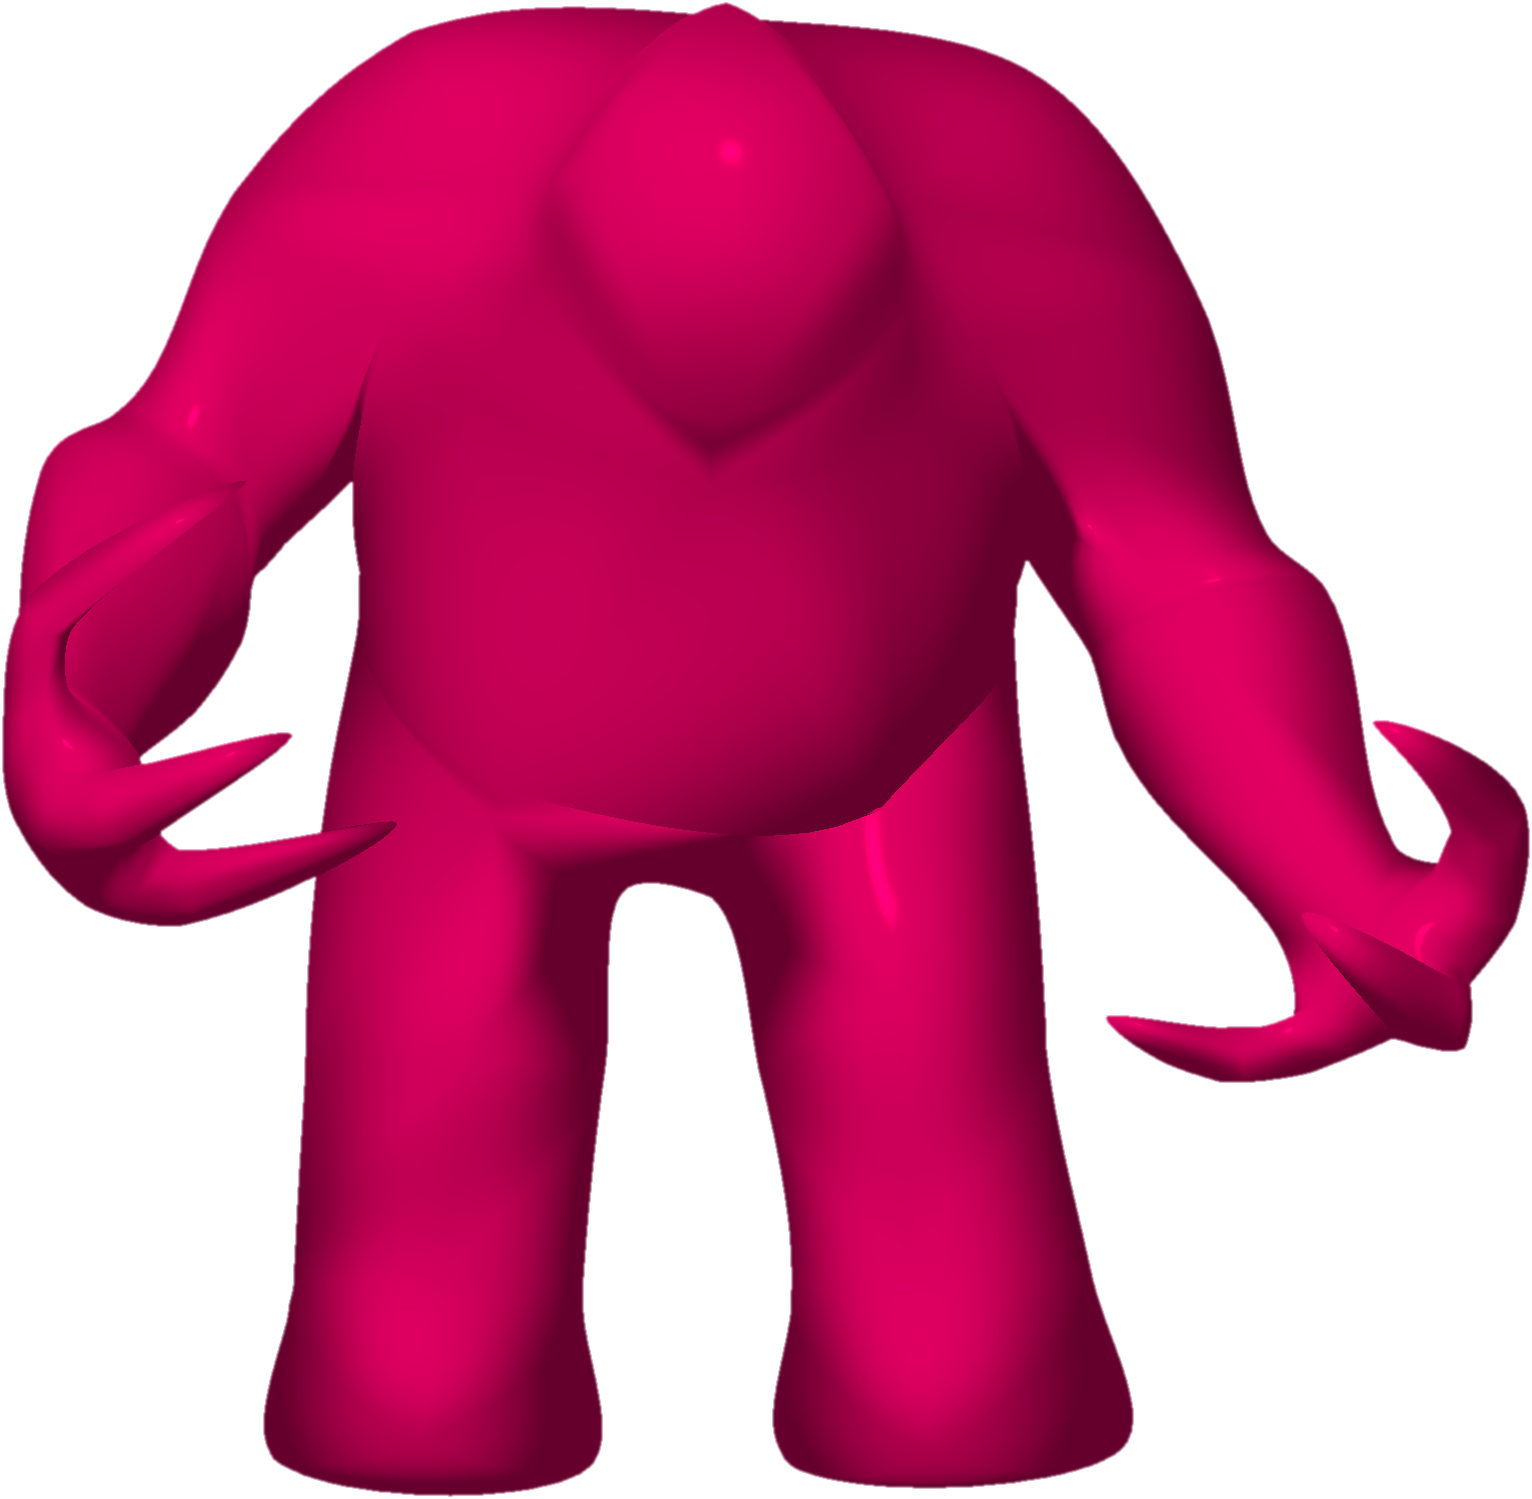
\includegraphics[width=\textwidth]{content/img/results/cpugpu/shamblerGPU.png}
		\caption{Shambler on GPU}
		\label{fig:results:cpugpu:gpuShambler}
	\end{subfigure}			
	\caption{A family of game characters from the game Quake 1. \Cref{fig:results:cpugpu:cpuDog,fig:results:cpugpu:cpuVore,fig:results:cpugpu:cpuShambler} are rendered on a CPU by \citeauthor{vlachos2001curved}. \Cref{fig:results:cpugpu:gpuDog,fig:results:cpugpu:gpuVore,fig:results:cpugpu:gpuShambler} are rendered by our implementation. We rendered our models with the Phong shading and reflection model ($k_s = 0.3$, $k_d = 0.5$, $k_a = 0.4$, $\alpha = 150.0$, color = $(0.988, 0.0, 0.427)$), with a single light source $\left(I_s = I_d = I_a = (1.0, 1.0, 1.0)\right)$ at $(-2.0, 5.0, -10.0)$. The inner and outer tessellation levels were set to $12.0$. The eye was placed at $(2.0, 5.0, -10.0)$.
% 
	\Cref{fig:results:cpugpu:cpuDog,fig:results:cpugpu:cpuVore,fig:results:cpugpu:cpuShambler} were taken from \textcite{vlachos2001curved}.}
	\label{fig:results:cpugpu}
\end{figure*}

%!TEX root = ../main.tex

\section{Conclusion}
\label{s:conclusion}
	It seems as computing rendering point-normal triangles on the GPU gives the same results as when the CPU, in spite of the different tessellation algorithm. However to accurately determine the influence, if any, of the tessellation algorithm on the final rendering on should implement point-normal triangles on both the CPU and the GPU. This would give full control over the used models and the shading parameters. This ensures that any differences between models rendered on the CPU and the GPU are due to the different tessellation algorithms.

	Although `real' normals result in the same normal as `fake' normals it is computationally advantageous in nearly all cases to use the `fake' normals. Only when one renders an object with point normal triangles with the level of detail set to 0, i.e. the inner and outer tessellation levels are 1.0, is it computationally advantageous to use `real' normals.

\printbibliography

\end{document}